
\chapter{Deployment of a Digital DAQ for a P-PC detector at Soudan Underground Laboratory}
\label{chap:DeploymentPPC2Soudan}
	\section{Introduction}
	\label{sec:DeploymentPPC2SoudanIntro}
			
		A PPC detector (henceforth referred to as PPC2) was procured by Pacific Northwest National Laboratory in January 2008 to be used in studies aimed at more clearly understanding the detector technology~\cite{Orr2007}.  Initial tests took place in the laboratory, focusing on basic operation and pulse-shape analysis techniques relevant for background reduction in the $\nonubb$ region-of-interest and for dark matter searches~\cite{Orr2008}.  In November 2008, PPC2 was deployed underground at Soudan Underground Laboratory at a depth of 2100~m.w.e.  The goals of this deployment were two-fold: (1) demonstrate the reliability and operation of a scaled-down \MJ-like digital DAQ system in an underground environment, and (2) investigate the possibility of obtaining Dark Matter exclusion data.  The latter goal was uncertain due to the lack of knowledge of the intrinsic backgrounds of the detector and its cryostat.  The development of the DAQ system used in this deployment is outlined in Chapter~\ref{chap:DAQDevel}
		
		Underground, the detector was placed inside 8~inches of Pb with a 2-inch inner shield composed of OFHC Cu.  This shield was surrounded by a sealed radon-exclusion box over-pressurized with nitrogen gas from LN boil-off to limit the introduction of Rn gas.  Borated-polyethylene planks were built up surrounding this for moderation of neutrons generated by interactions of cosmic-ray muons in the rock walls.  An engineering drawing of the shield can be seen in Figure~\ref{fig:PPC2OnlyShield} and with all components in Figure~\ref{fig:PPC2Shield}.  Relevant characteristics of the crystal are given in Table~\ref{tab:PPC2Characteristics}.
	
			\begin{figure}
				\centering
				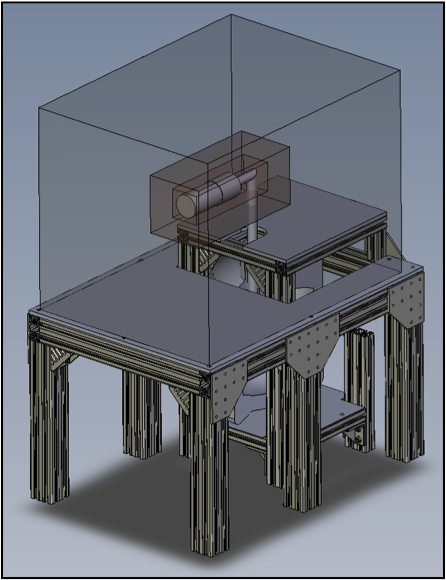
\includegraphics[width=0.6\textwidth]{PPC2DesignSchematicShield}
				\caption[Engineering drawing of PPC2 deployment]
				{Engineering drawing of the setup including inner and outer Cu and Pb shields which rests upon the frame.
				Graphic courtesy of J.~Orrell and E.~Fuller.}
				\label{fig:PPC2OnlyShield}
			\end{figure}
	
			\begin{figure}
				\centering
				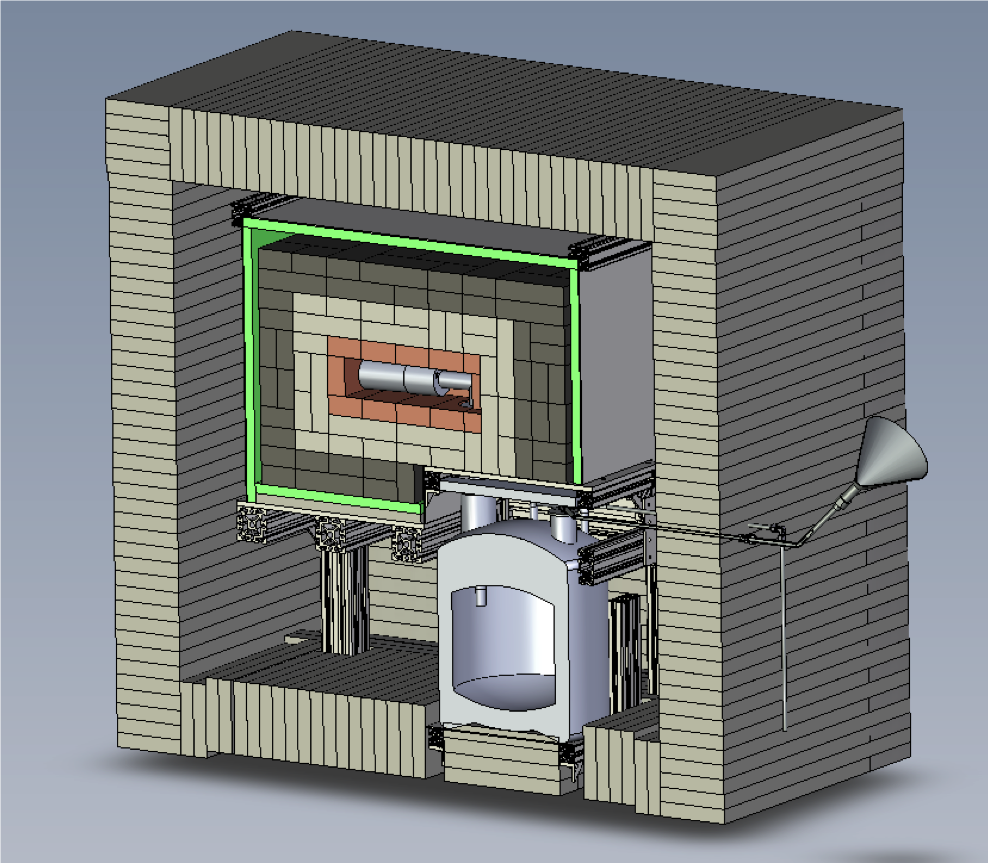
\includegraphics[width=0.9\textwidth]{PPC2DesignSchematicAll}
				\caption[Engineering drawing of PPC2 deployment, detailing outer components]
				{Engineering drawing of the setup including inner and outer Cu and Pb shields, Rn exclusion box, 
				and outer neutron moderator.  Graphic courtesy of J.~Orrell and E.~Fuller.}
				\label{fig:PPC2Shield}
			\end{figure}
	
			\begin{table}
				\centering
				\begin{tabular}{l|r}
					Property & Value \\
					\hline
					\hline
					Mass & 528 g \\
					Outer diameter & 50.1 mm \\
					Length & 50.3 mm \\
					\hline
					\hline
				\end{tabular}
				\caption[PPC2 detector characteristics]
				{PPC2 detector characteristics.  }
				\label{tab:PPC2Characteristics}
			\end{table}
	
	\section{Description of DAQ system}
	\label{sec:DeploymentPPC2SoudanDAQSystem}
	
	The DAQ system was designed as a single-channel prototype for the \MJ~\minmod.  Additionally, a significant amount of effort was put in to ensure that the setup was remotely configurable to enable the modification of experimental parameters from experimenters at the University of Washington and PNNL.  Signals from the detector were read out using a Gretina Mark IV digitizer designed by the GRETA collaboration~\cite{Anderson:2009p1293}.  This VME64x-based ADC digitized 10 independent channels at 100~Ms/s with a resolution of 14 bits.  The card was read out on the VME backplane using a Concurrent Technologies VX 407/042 Single-board computer controlled via gigabit ethernet by the ORCA DAQ and slow controls software~\cite{ORCA} running on an Apple Mac Mini computer.  For more details regarding the ORCA DAQ software and the development of its components relevant to this hardware configuration, please see Appendix~\ref{app:ORCASoftwareChapter}.  Also, additional details regarding the development and investigation of this DAQ system are given in Chapter~\ref{chap:DAQDevel}. The high voltage on PPC2 was controlled via a Canberra LYNX system which allowed for remote powering on and off of the detector bias.  The Liquid Nitrogen (LN) dewar was filled manually by the laboratory staff so no explicit tag was set in the data stream during these fills.  Techniques to cut out these events are discussed in Section~\ref{sec:DeploymentPPC2SoudanAnalysisCuts}.
	    
	As with most low-noise designs, the PPC2 preamp employed a pulse-reset circuit to avoid the Johnson noise associated with a feedback resistor.  The preamp had 3~outputs: 2~signal outputs and 1~inhibit output which would fire when the reset circuitry of the preamp was active.  Additionally, there was a test input for pulser signals used in electronic testing.  The 2~signal outputs were AC-coupled to remove their DC components using independent capacitors of $\sim500$~nF to yield a roughly 50~$\mu$s decay time of the preamp pulses.  One of these channels was input directly into the digitizer; the other was routed through a Phillips Scientific 777 fast amplifier (DC$\to$200~MHz bandwidth) with roughly $10\times$ gain to obtain better resolution near threshold.  The signal was split after the 777, with one output being input into the Gretina card and the other routed through a conventional spectroscopy amplifier (Ortec 667) to generate the trigger for the high-gain channel.  Figure~\ref{fig:PPC2DAQSetup} provides a simplified visualization of the DAQ setup including signal paths.  See Section~\ref{sec:DeploymentPPC2SoudanTriggerDesign} for more details regarding the high-gain trigger and its development.  The inhibit output was sent directly into the Gretina digitizer card to record the timing information of the reset circuitry.
	
	The test input of the preamp was used for pulser signals to measure the efficiency of the trigger.  The pulser used was an Agilent 33220A waveform generator controlled via ethernet by ORCA running on the Mac mini.  The pulser output passed through 2~computer-controlled attenuators (HP 8494/5G, 0$\to$4~GHz bandwidth) to get up to 71~dB of attenuation in increments of 1~dB.  These attenuators were actuated using a constructed driver box controlled with an InterPak 408 digital I/O card on the VME bus.  For more details on the pulser test setup, see Section~\ref{sec:DeploymentPPC2SoudanTriggerDesign}.  A synchronization pulse from the Agilent was input directly into the digitizer for timing information.  The pulser was also used during counting runs, inputting a signal of low amplitude, $\sim$2.5~keV, into the DAQ system at low rate $\sim1$~Hz, with the purpose to measure any deviations in the electronics over time.
		     
	A summary of the input channels on the Gretina card including the type of data saved for each is given in Table~\ref{tab:PPC2DAQChannelInfo}.  
%A schematic of the DAQ setup is shown in Figure~\ref{fig:PPC2DAQSetup}.  
The DAQ system was fully deployed underground at the beginning of April 2009.
		 
			\begin{table}
				\centering
				\begin{tabular}{l|c|c}
					Type & Channel &  Info \\
					\hline
					\hline
					Reset inhibit & 9 & Only timing \\
					\hline
					Low-gain signal & 8 & 10~$\mu$s trace (1022	 samples) \\
					\hline
					Pulser sync & 7 & Only timing \\
					\hline				
					Muon veto & 2 & Only timing, unused in analysis \\
					\hline								
					High-gain trigger & 1 & Only timing \\
					\hline								
					High-gain signal & 0 & 10~$\mu$s trace (1022 samples) \\				
					\hline
					\hline
				\end{tabular}
				\caption[Channel summary for the Gretina digitizer card]
				{Channel summary for the Gretina digitizer card.  }
				\label{tab:PPC2DAQChannelInfo}
			\end{table}	     
	
	
			\begin{sidewaysfigure}
				\centering
				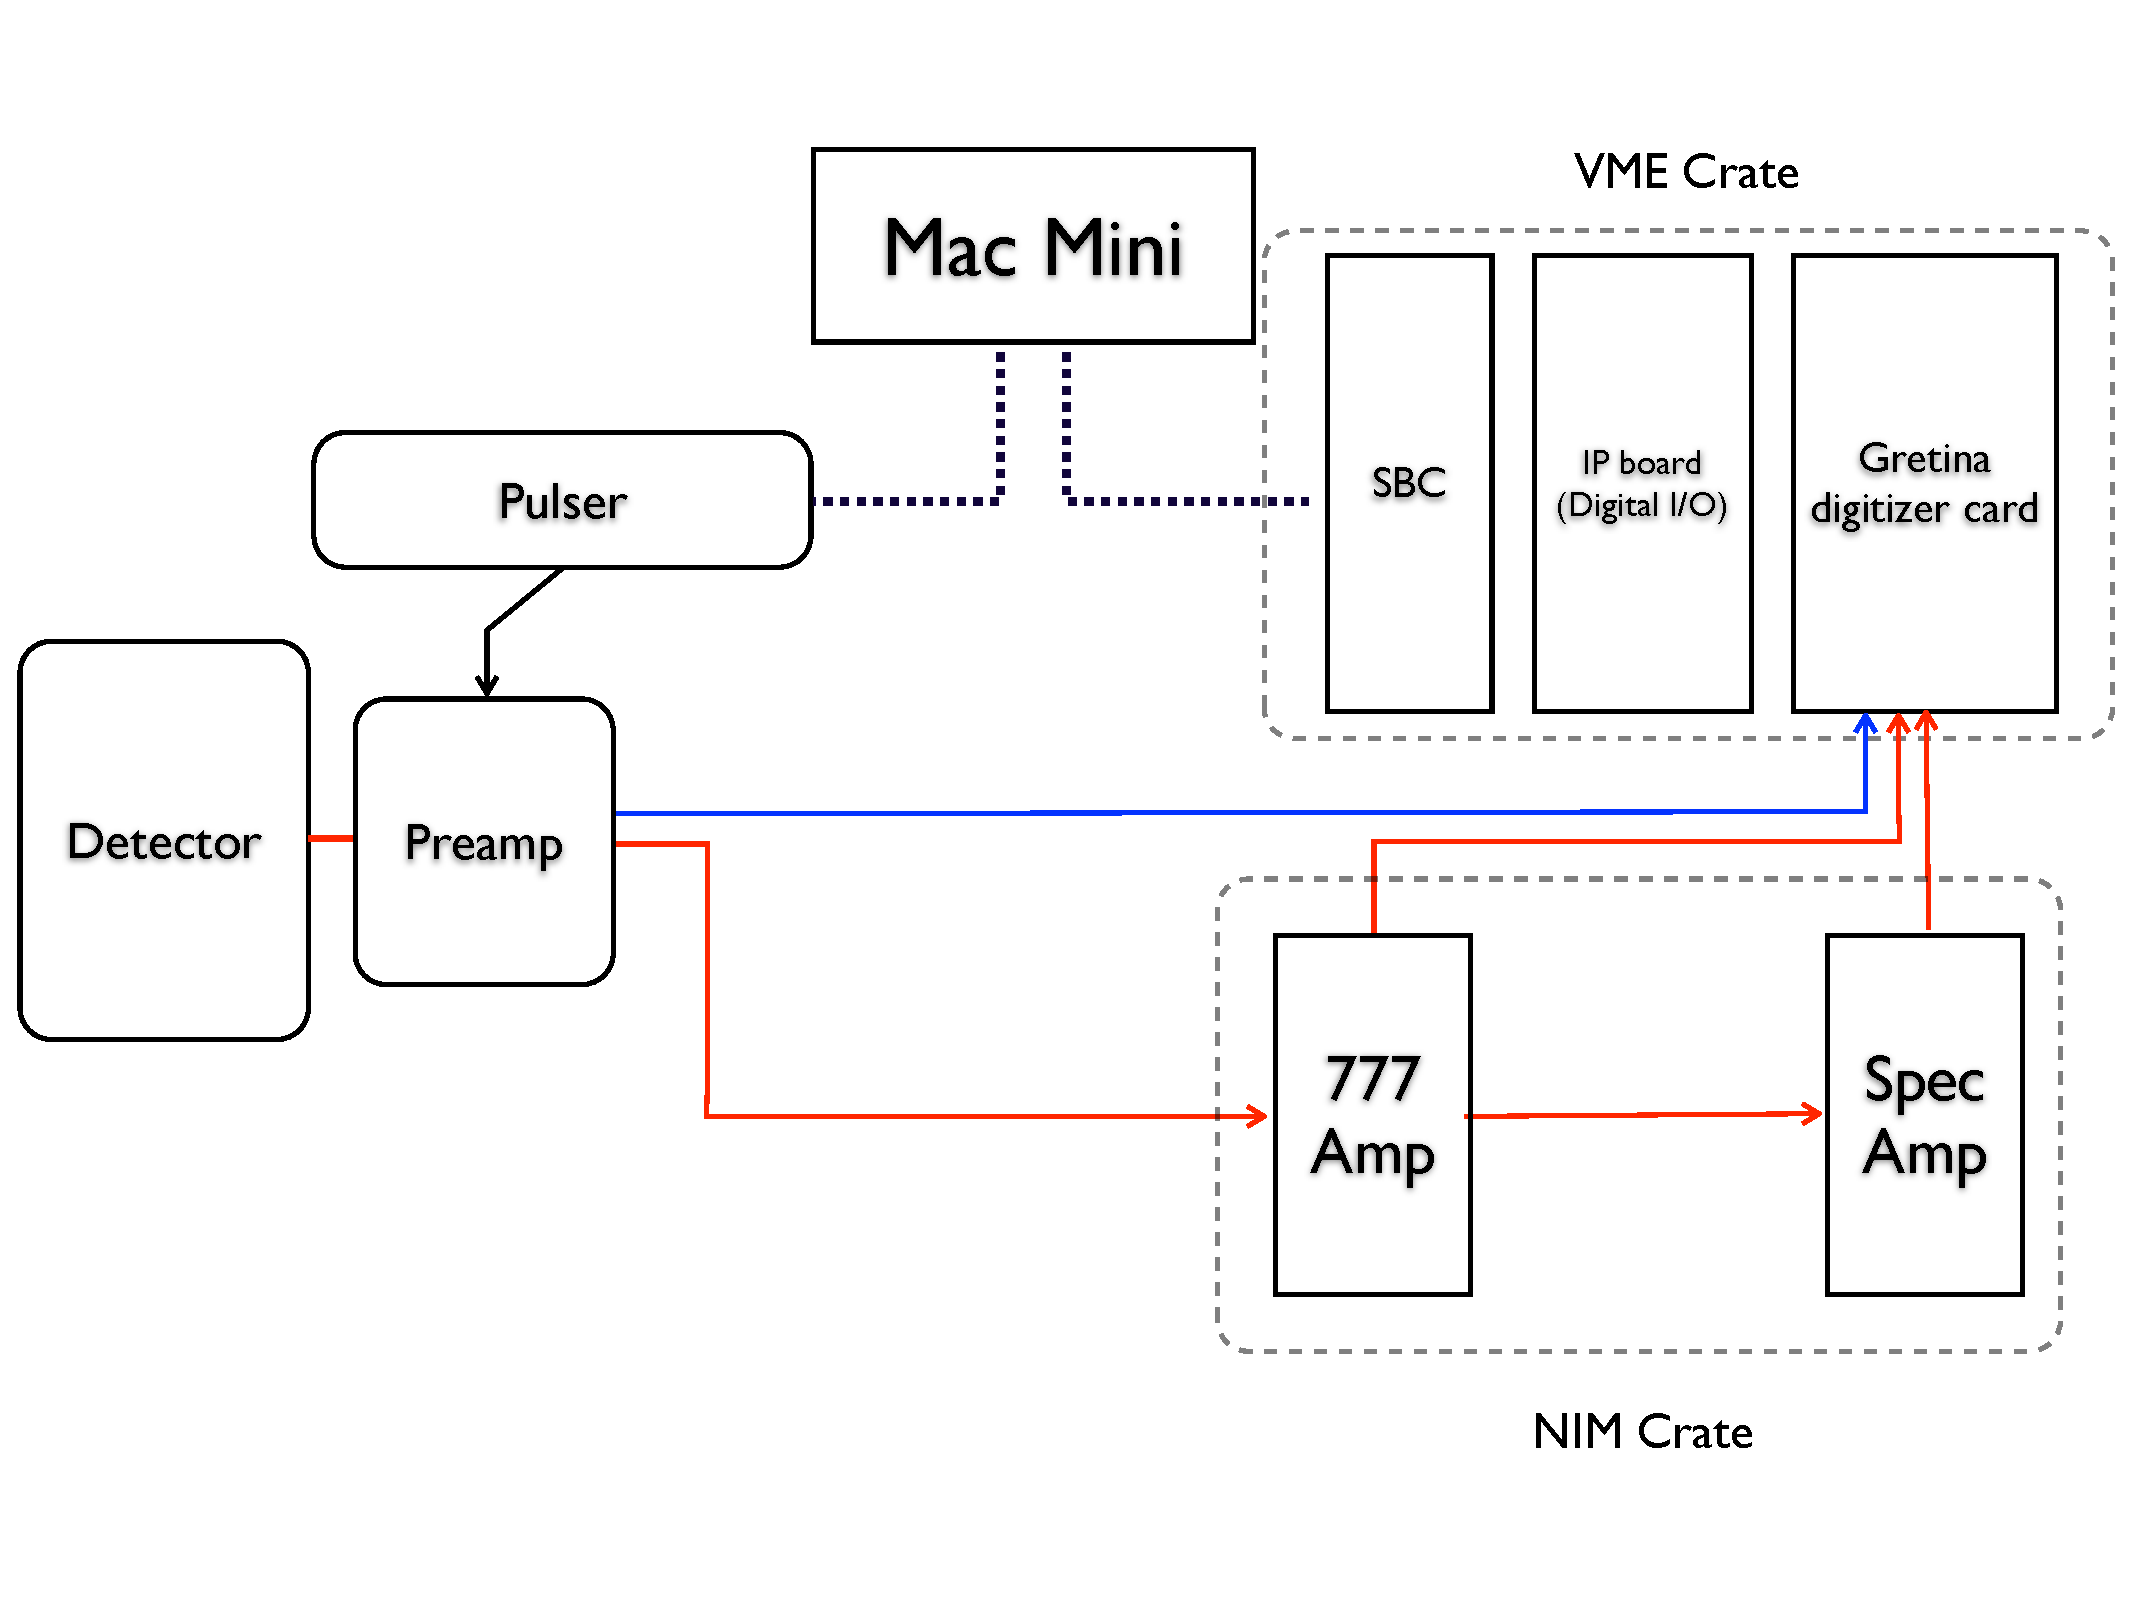
\includegraphics[width=0.95\textwidth]{PPC2DAQSchematic}
				\caption[Simplified schematic of DAQ setup] 
				{Simplified schematic of DAQ setup.  Lines with arrows denote signal flow.}
				\label{fig:PPC2DAQSetup}
			\end{sidewaysfigure}
		     			
	\section{Analysis and Results}
	\label{sec:DeploymentPPC2SoudanAnalysis}
	
	After a few months of commissioning and calibration tests, counting runs were begun on 3 May 2009.  Runs were cycled every hour, and data was automatically synchronized with a server at the University of Washington.  On 10 June 2009, automatic trigger efficiency tests were begun in between runs to monitor the stability of the trigger over time.  Counting runs ended on 24 July 2009, yielding a total live-time of 70.4 days.  A CouchDB database~\cite{CouchDB} was used to store both metadata (e.g.~timing, configuration, file names, etc.) as well as analysis parameters (e.g.~average baseline, trigger efficiency, measured electronic noise) from each run.  This database was also used to facilitate the analysis chain described in the following section.    

		\subsection{Data processing}
		\label{sec:DeploymentPPC2DataProcessing}	
	
	All data was handled in a tiered reduction scheme.  The analysis process was automated and made significant use of the ROOT analysis framework~\cite{Bru97} as well as waveform analysis tools (MGDO, see Appendix~\ref{app:MGDO} for more information) developed for the \MJ~experiment.  An outline of the tiered data-flow process is given:
		\begin{description}\itemsep2pt
			\item[Tier 0:]  Raw binary data -- from the ORCA DAQ system
			\item[Tier 1:]  ROOTified data -- raw data converted to MGDO objects and stored in ROOT TFiles
			\item[Tier 2:]  Waveform processed data -- extraction of waveform characteristics using MGDO Transforms
			\item[Tier 3:]  Reduced and split data
		\end{description}	
		
	This process was tracked using a CouchDB database.  The Tier~$0\to1$ conversion process took the raw binary data and converted it into MGDO \cpp~objects which could then be serialized to disk in ROOT TFiles.  The Tier~$1\to2$ processing calculated several parameters from the waveform data, including baseline, extrema (maximum and minimum), and rise-time and determined the amplitude of the waveform using a trapezoidal filter\footnote{The Gretina digitizer included an on-board trapezoidal filter, but it was chosen to use an offline filter for greater flexibility.}~\cite{Jor94}.  More information regarding the baseline and rise-time calculations are given in Sections~\ref{sec:DeploymentPPC2SoudanAnalysisCuts} and~\ref{sec:DeploymentPPC2SoudanAnalysisRisetime}.  Additionally, at this stage coincidences between events in different channels were calculated using the timing information from the digitizer card, defining events within $1~\mu$s of each other as concurrent.   Finally, the Tier~$2\to3$ processing reduced the data size, removing noise events (i.e.~events well below energy threshold) and splitting the two signal channels 0 and 8 into separate file groups.  The Tier~3 files were used directly in analysis and made available to others in the \MJ~collaboration through a cloud-based file system (Dropbox\footnote{See the Dropbox website: \url{https://www.dropbox.com} for more information.}).
	
		\subsection{Initial calibration}
		\label{sec:DeploymentPPC2SoudanAnalysisCalibration}    
			
	The system was initially calibrated with a $^{133}$Ba source using peaks detailed in Table~\ref{tab:Ba133Peaks},~\cite{Rab1995491}.  The high- and low-gain channels were calibrated independently and spectra for each channel are shown in Figure~\ref{fig:PPC2Calibration}.  These initial calibrations were used for commissioning tests such as trigger efficiency and electronic noise measurements and were later refined using prominent peaks from backgrounds e.g.~in the U and Th chains, $^{40}$K, and x-ray lines from \gersixeight~and \znsixfive~electron capture decays (see Section~\ref{sec:DeploymentPPC2SoudanAnalysisEnergySpectra}).  During the counting runs, regular calibration runs were not made; instead we monitored the behavior of the detector using an injected pulser.  

				\begin{table}
					\centering
					\begin{tabular}{l|r}
						Energy (keV) & Intensity \\
						\hline
						    53.16 	 &     2.2 \% \\ 
						    79.61 	 &     2.62 \% \\
						    80.997 	 &    34.1 \%\\
						   160.61 	 &     0.65 \%\\
						   223.24 	 &   0.45 \% \\
						   276.4 	 &     7.16 \% \\
						   302.85 	 &   18.33 \% \\
						   356.01 	 &    62.05 \% \\
						   383.85 	  &    8.94 \% \\
						\hline
					\end{tabular}
					\caption[Selected gamma lines used for calibration in the $^{133}$Ba spectrum]
					{Selected gamma lines used for calibration in the $^{133}$Ba spectrum, 
					data adapted from~\cite{Rab1995491}.}
					\label{tab:Ba133Peaks}
				\end{table}	
						
				\begin{figure}
					\centering
					\subfigure[High-gain channel]{
						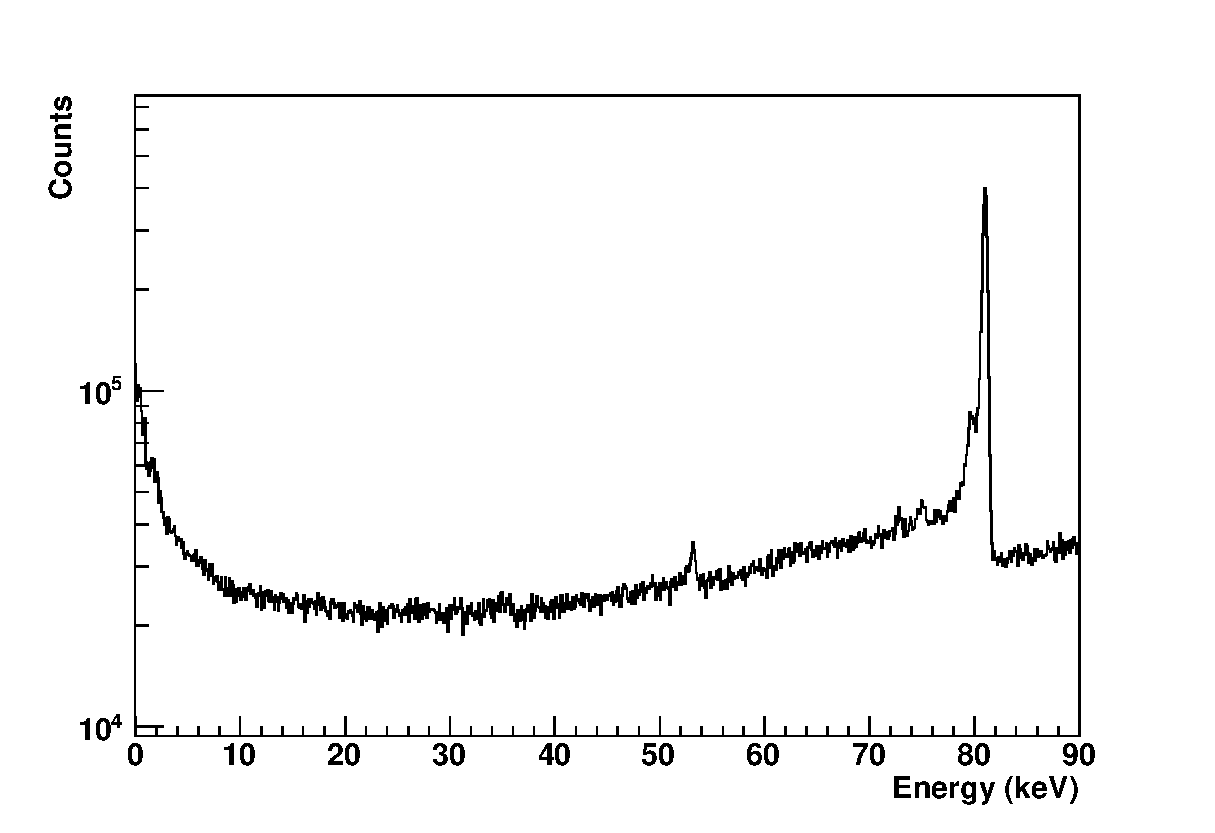
\includegraphics[width=0.9\textwidth]{LowEnergyCal}
						\label{fig:PPC2CalLow}
					}
					\subfigure[Low-gain channel]{
						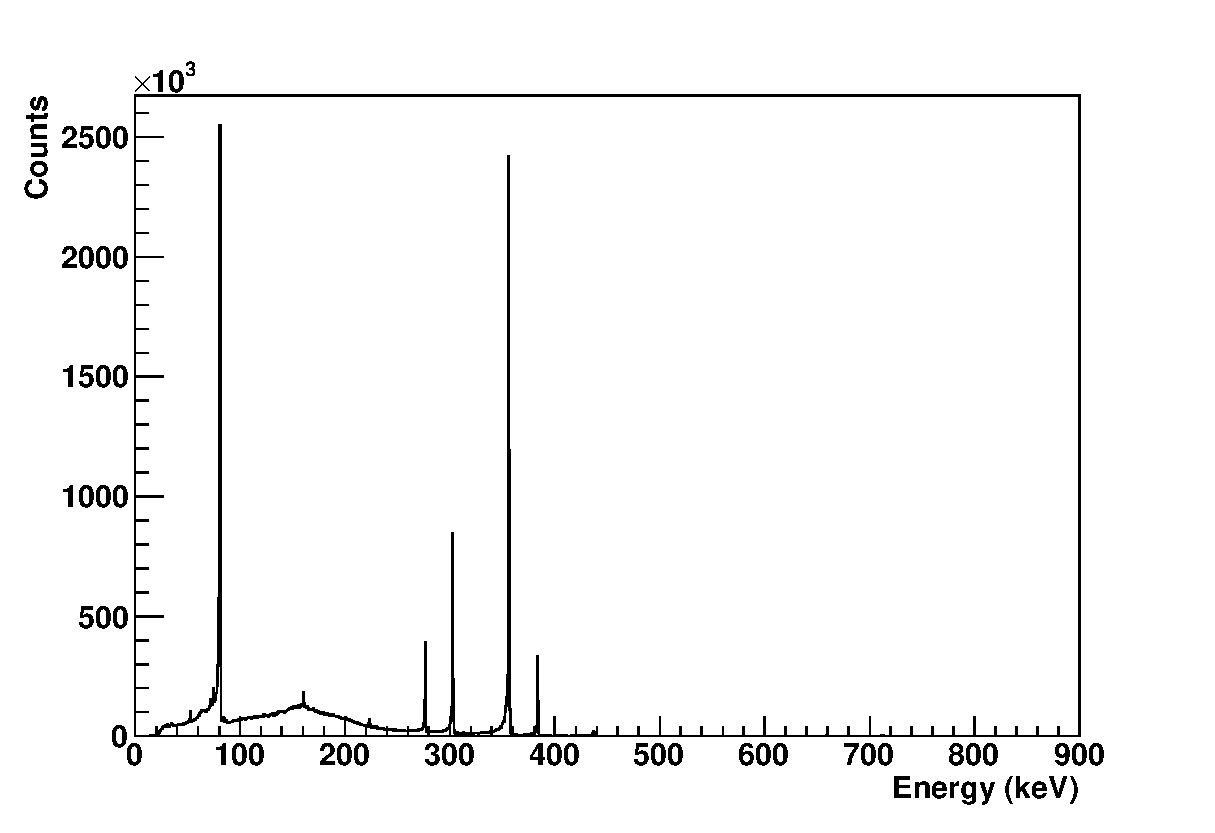
\includegraphics[width=0.9\textwidth]{HighEnergyCal}
						\label{fig:PPC2CalHigh}
					}
					\caption[Calibration of the high- and low-gain channels]
					{Calibration of the high- and low-gain channels.}
					\label{fig:PPC2Calibration}
				\end{figure}

		\subsection{Detector parameters vs.~time}	
		\label{sec:PPC2DetParsVsTime}
		
	Several parameters of the system were tracked over time, including the trigger efficiency and the electronic noise of the system.  The former was tested by performing efficiency tests every hour in between run cycles; the latter by looking at the recorded data of the input pulser pulses (1~Hz) versus time.  Several other parameters, including the baseline of the waveforms and the number of events in a certain energy ranges, were tracked as well: these results are presented in Section~\ref{sec:DeploymentPPC2SoudanAnalysisCuts}.  In addition to these specific parameters being tracked, the rates of each channel were tracked.  While tracking these rates, it was determined that the reset rate of the preamp increased towards the end of an LN fill cycle.  Higher values of inhibit rate (lower baseline values) occurred as LN in the dewar boiled off, with sharp returns when the dewar was refilled.  The interpretation of this was that as the level of LN in the dewar fell, the temperature of the front-end detector electronics (and possibly the crystal) would increase which would increase the detector leakage current.  An increase in leakage current would cause the preamp to reset more often to clear the charge more quickly accumulating on the feedback capacitor.  It was not determined precisely what caused this temperature sensitivity; however, it was likely due to insufficient thermal coupling between the detector and the liquid nitrogen.  During installation of the detector within the Pb shield, an extension had to be added to the dewar end of the cold finger.  It is possible that this extension didn't properly thermally couple to the cold finger and thus didn't cool the detector and/or the internal electronics as effectively.  The change of the reset rate over time had implications for other parameters as discussed in the following sections.  A summary of comparisons between detector parameters is shown in Figure~\ref{fig:PPC2AllPlotCompare}.  In this figure, LN fills occurred around runs~1590, 1665, and 1750.  The average values of the parameters in the following sections is given in Table~\ref{tab:PPC2AvgPars}.
	
	

		    	\subsubsection{Pulser data}
			\label{sec:DeploymentPPC2SoudanAnalysisPulserData}    

	Pulses from the Agilent waveform generator were input into the test input at a rate of 1~Hz and at low energy: $\sim2.5$~keV.  These events underwent analysis equivalent to every other waveform and were selected by finding all waveforms which arrived in coincidence with the pulser synchronization signal.  Each hour-long run yielded a data set of $\sim3600$ events; the calculated amplitudes (energies) of these events were histogrammed and fit to a gaussian to extract the mean, $\mu$, and the sigma, $\sigma$, of the pulser signal for each run.  Results of these fits are plotted versus run number in Figure~\ref{fig:PPC2AllPlotCompare}.  It is clear that the width of the noise ($\sigma$) did not significantly alter for reset rates below 15~Hz.  However, the mean ($\mu$) of the pulser demonstrated three clear transition regions an example of which have been labeled `I', `II', and `III' in Figure~\ref{fig:PPC2AllPlotCompare}: from reset rates 3$\to$7~Hz (region I labeled in the plot), the mean increased, transitioned to lower values for reset rates 7$\to$11~HZ (region II), and then returned for rates above 11~Hz (region III).  The absolute cause of this behavior was not determined, but it is possibly due to a modification of operating parameters of the front-end crystal electronics (e.g.~the FET) by the increasing leakage current.  

			%%%%\begin{figure}
			%%%%	\centering
			%%%%	\subfigure[Pulser sigma, $\sigma$, vs.~time.]{
			%%%%		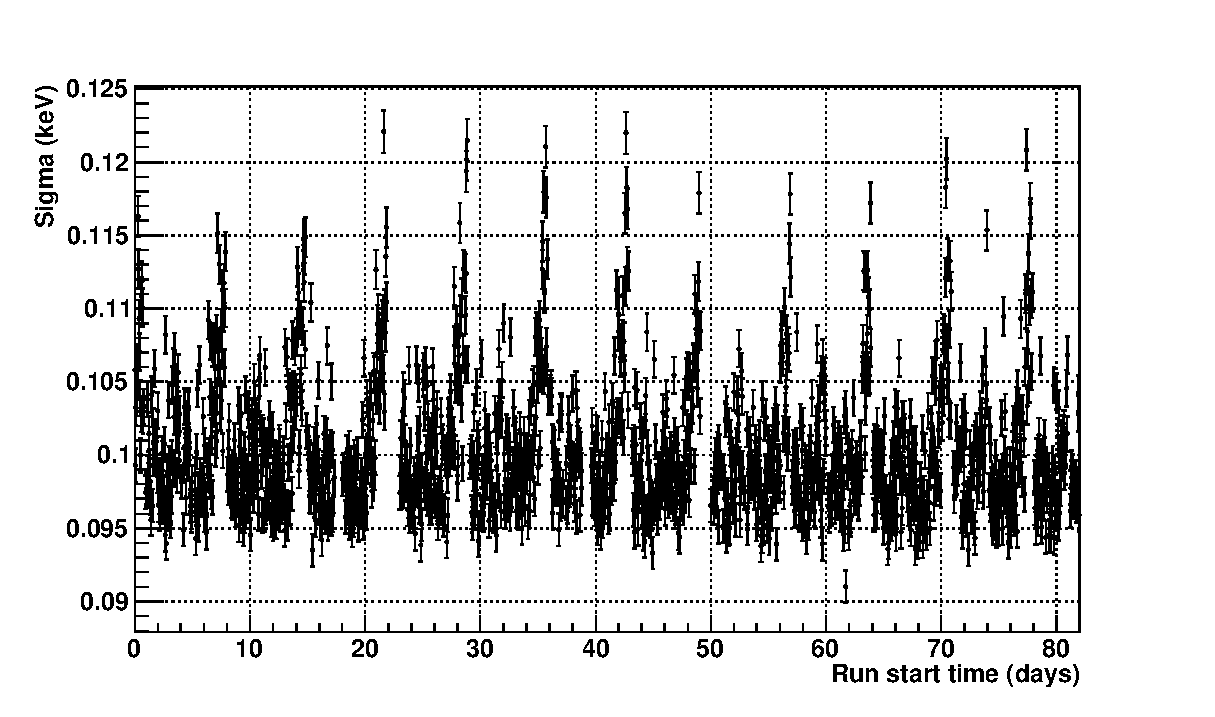
\includegraphics[width=0.45\textwidth]{PulserSigmaVsTime}
			%%%%	}
			%%%%	\subfigure[Pulser mean, $\mu$, vs.~time.]{
			%%%%		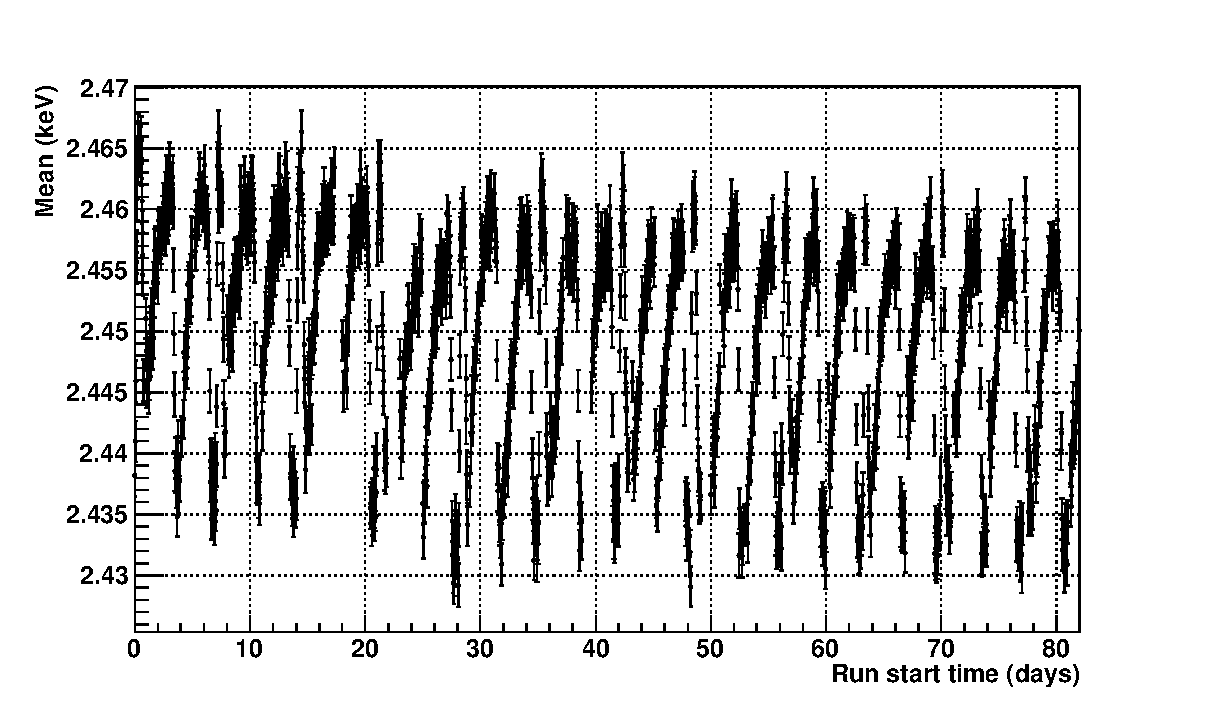
\includegraphics[width=0.45\textwidth]{PulserMeanVsTime}
			%%%%	}						
			%%%%	\caption{Measured $\mu$ and $\sigma$ of pulser versus run start time.}
			%%%%	\label{fig:PPC2PulserVsTime}
			%%%%\end{figure}



		    	\subsubsection{Trigger Efficiency}
			\label{sec:DeploymentPPC2SoudanAnalysisTriggerEfficiency}    
			
	Trigger efficiency was measured as described in Section~\ref{sec:DeploymentPPC2SoudanTriggerDesign}.  Initial tests were performed during the commissioning period (i.e.~before counting runs began) and automatic tests were run after every hour-long cycle beginning 38~days into the counting run period.  The goal of these tests was to investigate how the trigger threshold behaved over time, tracking any changes that might occur due to shifts in environmental conditions or because of other unforeseen phenomena.  To parameterize the efficiency, the data were fit to an error function, $f_{eff}(E)$, in the form:

				\begin{equation}
					f_{eff}(E) = \frac{1}{2} - \frac{1}{2} \operatorname{erf} \left( s ( E-\rho ) \right)
					\label{eqn:TriggerEfficiency}
				\end{equation}
				
with energy, $E$, in keV; scaling parameter, $s$, in keV$^{-1}$; and offset, $\rho$, in keV.  An example of a fit to this data is given in Figure~\ref{fig:PPC2TriggeringEfficiencyExample}.  Some results of the trigger tests over time are given in Figure~\ref{fig:PPC2AllPlotCompare}, comparing them to other detector parameters.  The offset parameter, $\rho$, was largely stable but increased before the transition from I$\to$II and again during region III.  $\rho$ returned to a lower value during region II.  The scaling, $s$, was largely insensitive to any change in reset rate, though exhibited slight deviations low in transitions between regions I and II.  

				\begin{figure}
					\centering
					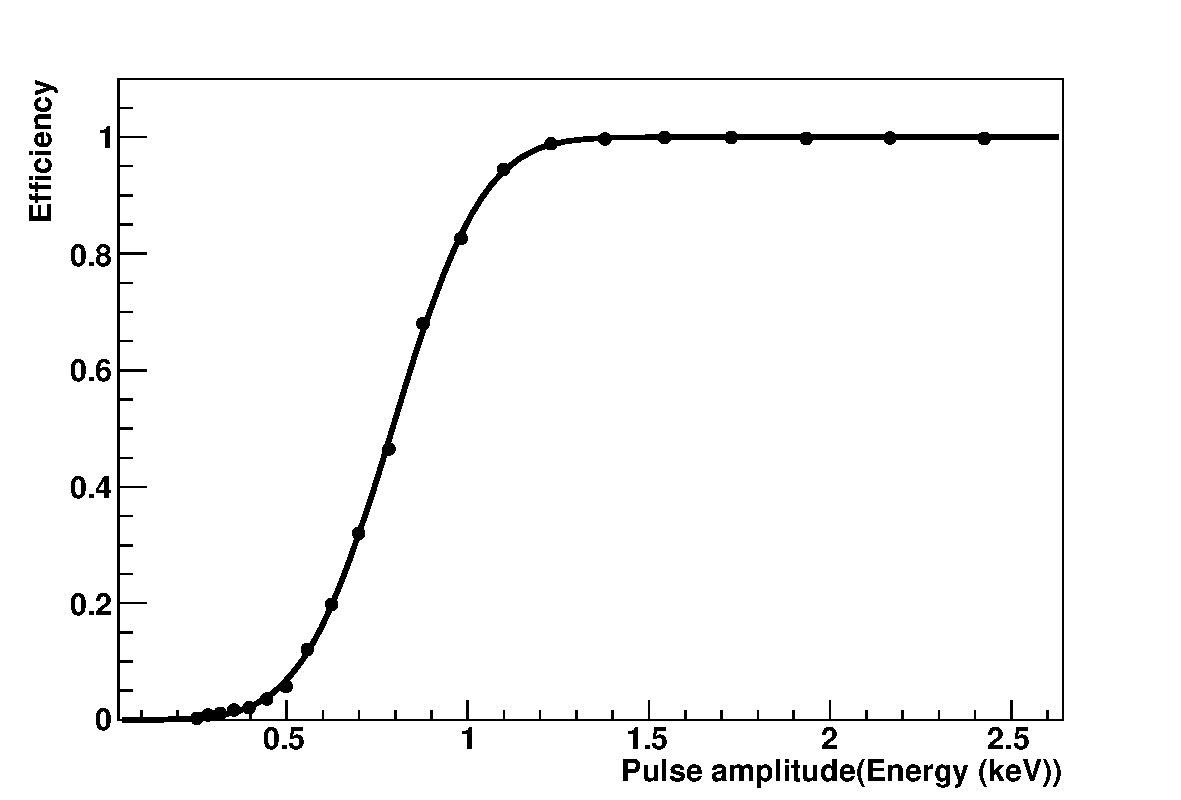
\includegraphics[width=0.7\textwidth]{EfficiencyExample}
					\caption[Triggering efficiency measurement example]
					{Triggering efficiency measurement example.  Line is a fit to 
					Equation~\ref{eqn:TriggerEfficiency}.}
					\label{fig:PPC2TriggeringEfficiencyExample}
				\end{figure}
	
			%%%%\begin{figure}
			%%%%	\centering
			%%%%	\subfigure[Scaling parameter, $s$, vs.~time.]{
			%%%%		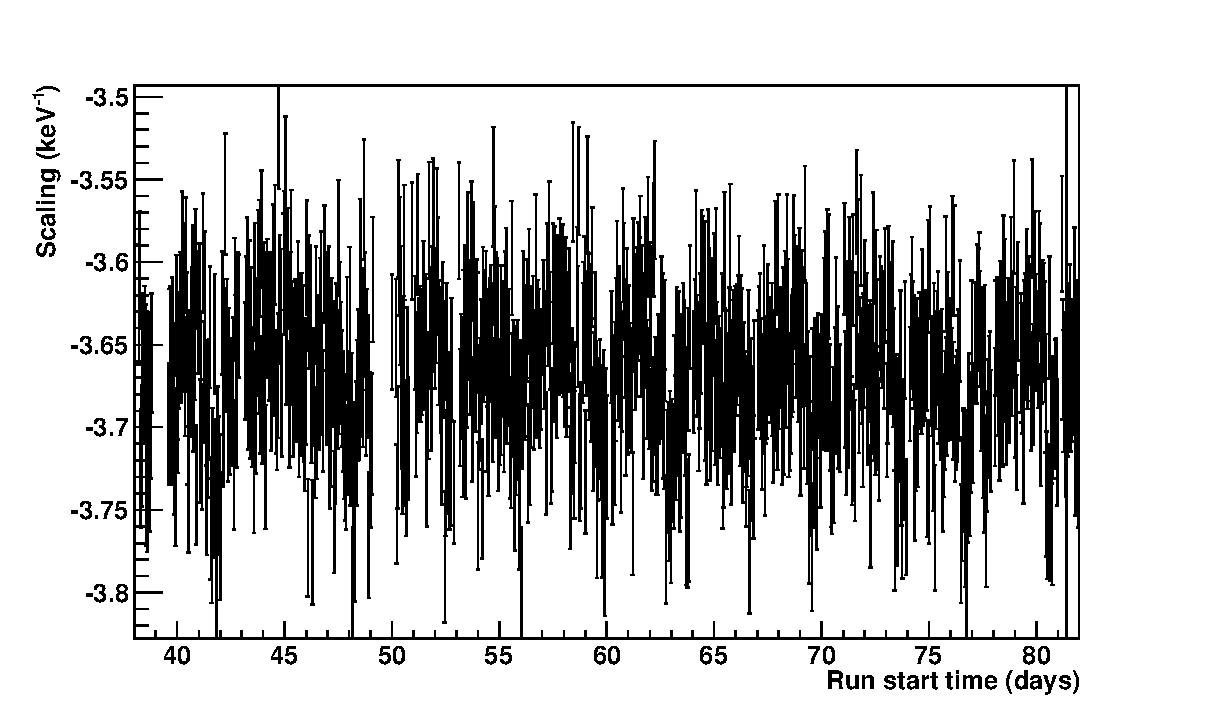
\includegraphics[width=0.45\textwidth]{ScalingVsRun0}
			%%%%		\label{fig:PPC2TriggeringEfficiencyTestsVsTimeScaling}
			%%%%	}
			%%%%	\subfigure[Offset parameter, $\sigma$, vs.~time.]{
			%%%%		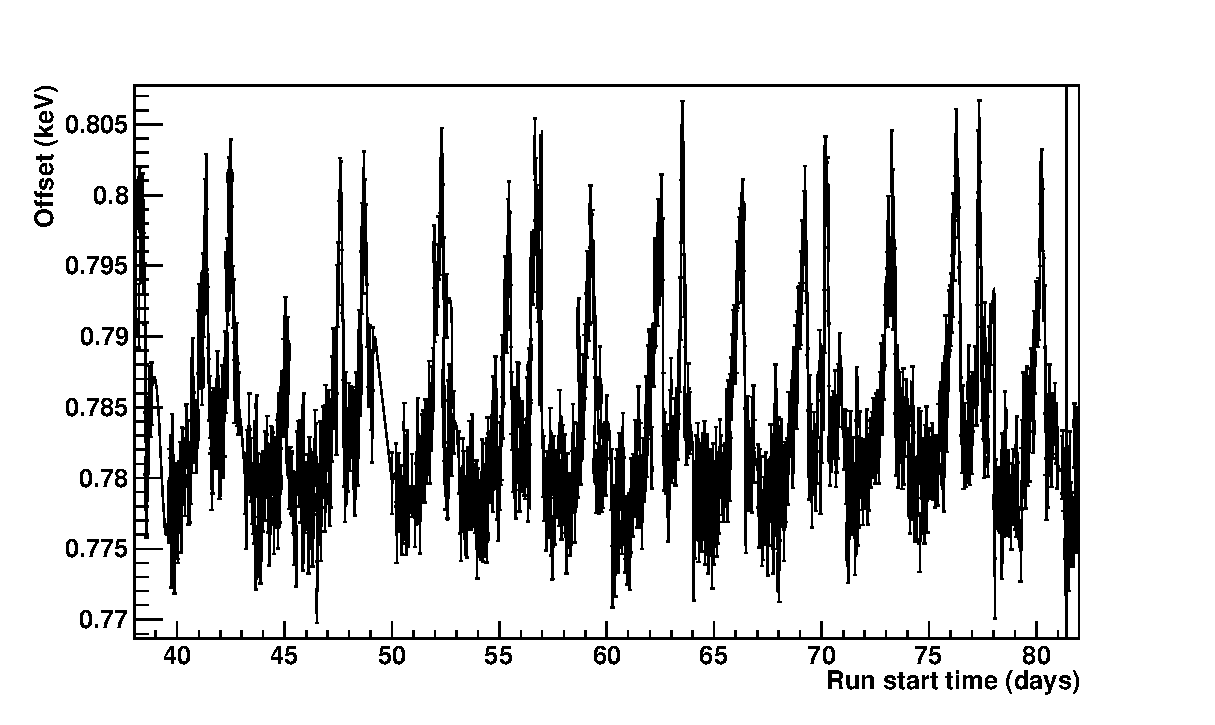
\includegraphics[width=0.45\textwidth]{OffsetVsRun0}
			%%%%		\label{fig:PPC2TriggeringEfficiencyTestsVsTimeOffset}
			%%%%	}						
			%%%%	\caption{Triggering efficiency tests vs. run time.  $\sim$5~min efficiency tests were run in 
			%%%%	between hour-long counting runs to measure how efficiency changed over time.}
			%%%%	\label{fig:PPC2TriggeringEfficiencyTestsVsTime}
			%%%%\end{figure}

			
				\begin{figure}
					\centering
					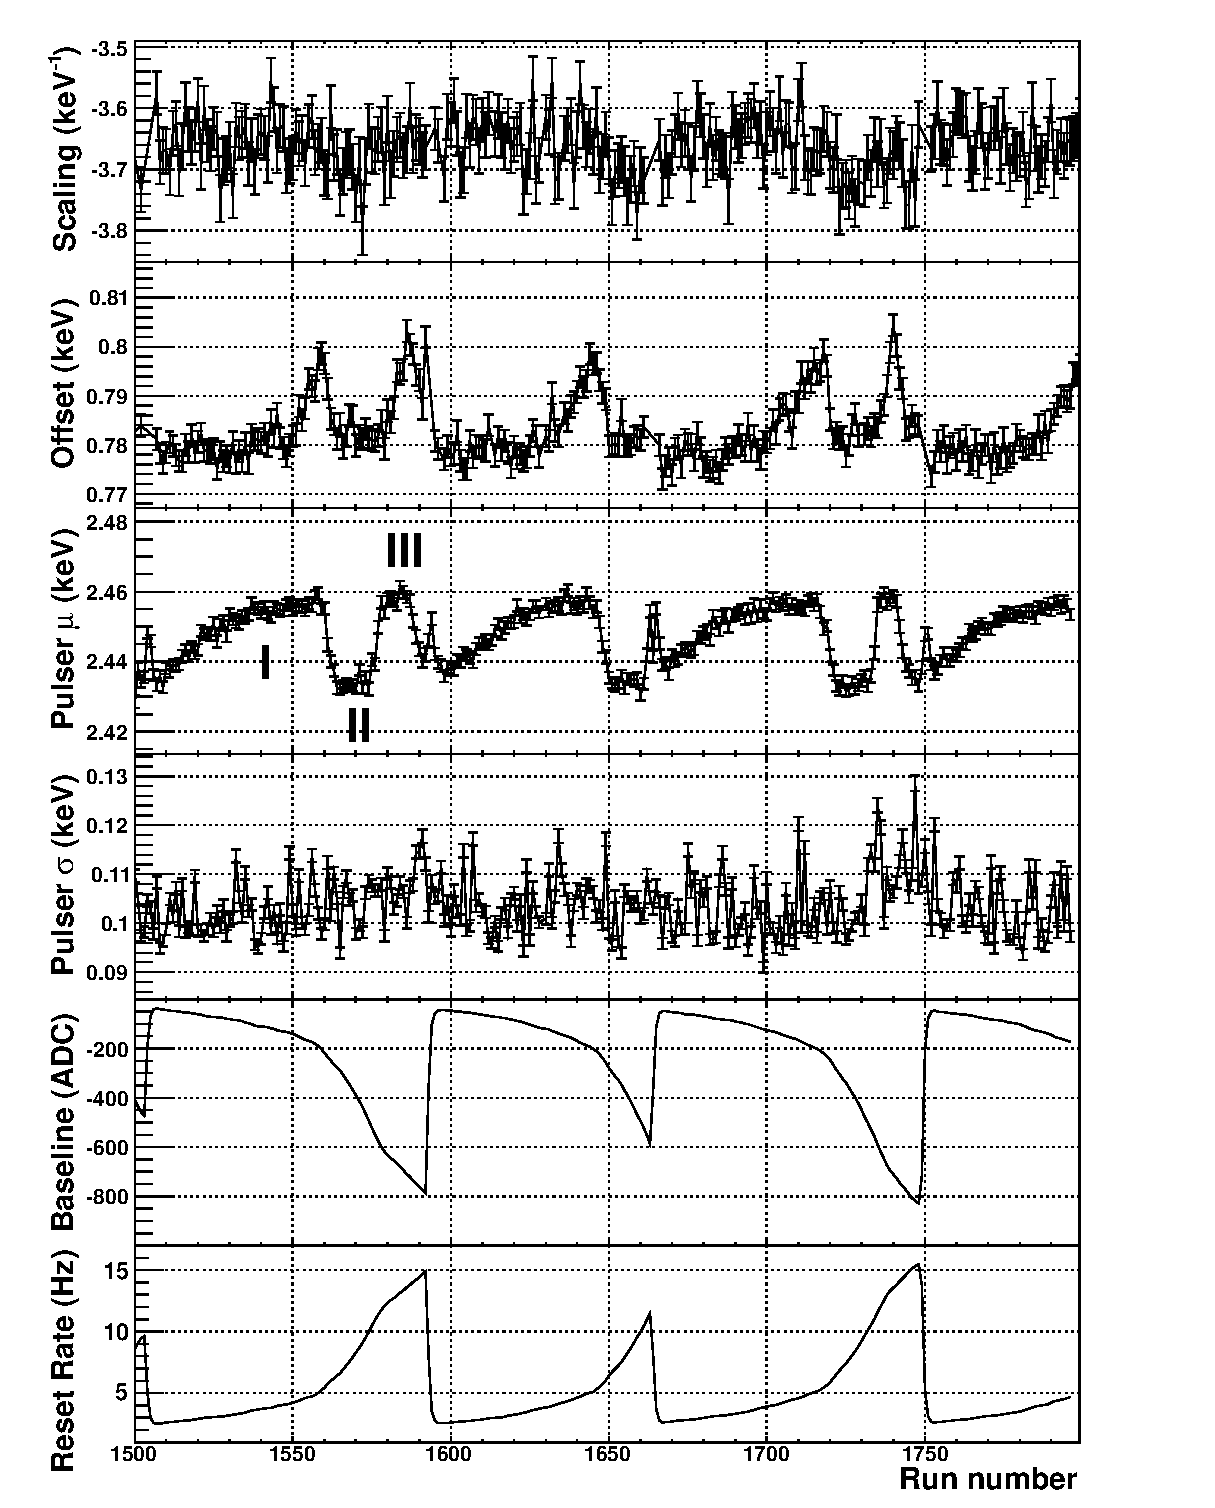
\includegraphics[width=0.95\textwidth]{AllPlotComparisons}
					\caption[Comparison of various parameters versus time for a subset of runs]
					{Comparison of various parameters versus time for a subset of runs.  See text for details.}
					\label{fig:PPC2AllPlotCompare}
				\end{figure}
	
	    	\subsubsection{Conclusions}
		\label{sec:DeploymentPPC2SoudanAnalysisParsTimeConclusion}    	
	
	The results of this section underscore the need to track detector parameters over time to monitor changing environmental conditions and other unanticipated behavior.  The gain and offset shifts evident in the pulser and trigger efficiency results do not significantly affect these data because their magnitudes ($<$25~eV) are much less than the nominal noise FWHM ($\sim$235~eV) and trigger threshold (90\% efficient at 1~keV) (see average values in Table~\ref{tab:PPC2AvgPars}).  However, these deviations could begin to have a larger effect with improved systems with reduced noise and threshold.  Additionally, when extracting information on physics signals in regions close to threshold (such as dark matter), it is critical to study parameters affecting this region over time to understand systematics important for limits or claims.  
	
				\begin{table}
					\centering
					\begin{tabular}{l|r}
						Parameter & Value \\
						\hline
						    Pulser Data 	  \\
						    Mean, $\mu$ &  $2.45\pm0.009$ (keV) \\
						    Sigma, $\sigma$ &  $0.100\pm0.0046$ (keV) \\						    
						    Trigger Efficiency 	  \\
						    Offset, $\rho$ &  $0.784\pm0.006$ (keV) \\
						    Scaling, $s$ &  $-3.666\pm0.044$ (keV$^{-1}$) \\						    						    
						\hline
					\end{tabular}
					\caption[Average parameters for trigger efficiency and electronic noise]
					{Average parameters for trigger efficiency and electronic noise.}
					\label{tab:PPC2AvgPars}
				\end{table}	
	    	\subsection{Cuts}
		\label{sec:DeploymentPPC2SoudanAnalysisCuts}    
			
	Cuts were introduced to clean the data with the goal of removing spurious events from, for example, noise, microphonics and reset-pulse events.  These consisted of (1) a timing cut for removing reset pulse events, and (2) a baseline cut and (3) an integrated-counts-per-run cut for removing noise and microphonics-induced events.  The first two cuts were applied on an event-by-event basis, whereas the last cut removed an entire hour-long run. 
	
			\subsubsection{Reset-pulse timing cut}
	Reset pulse waveforms had distinct qualities (positive clipping whereas energy pulses were negative-going) which allowed the waveforms to be removed online from the data stream while retaining the timing information of the event.  The offline timing cut introduced a veto window of 1~ms following a reset event.  Given the average reset rate ($\sim$10~Hz), this introduced a $\sim$1\% correction to the live-time.  

			\subsubsection{Baseline cut}	
	The baseline of the traces were monitored on an event-by-event basis by calculating a 1st-degree polynomial fit to the first 3.5~$\mu$s of each preamp trace.  From this information, an average baseline was calculated for each run to generate a cut based upon significant deviations from these average values.  In a stable system, the baseline will be gaussian distributed around a central value according to the magnitude of the noise.  The integrated-counts-per-run in particular energy windows (0.6-10~keV and 10-70~keV) were monitored as well to observe deviations from expectation assuming poisson statistics.  This second cut relied upon the fact that spurious events from increases in environmental noise and microphonics arrive in bursts, see e.g.~\cite{Morales1992410}).  
	
	The average baseline per run shifted with a systematic correlation with a shift in the measured inhibit rate, shown in Figure~\ref{fig:PPC2AllPlotCompare}.  As the leakage current increased, the inhibit rate went up and the measured baseline dropped due to additional charge collection on the AC-coupling capacitor.  In general, this downward shift in baseline could affect the dynamic (energy) range of a digitizer channel because it would allow fewer ADC values for the (negative-going) pulses before clipping.  To generate a cut on this value, the values of the baseline for each event during a run were histogrammed and fit to a gaussian.  A cut was then generated based upon the results of this fit: rejecting events outside the range $\mu\pm3\sigma$ for a 99.7\% acceptance.  An example of one of these fits is shown in~\ref{fig:PPC2BaselineCuts}.  During LN fills, the baseline would return to its maximum value making a cut based upon the average baseline value impossible.  Runs during these transition times were cut from the data set.  
		
			%%%%\begin{figure}
			%%%%	\centering
			%%%%	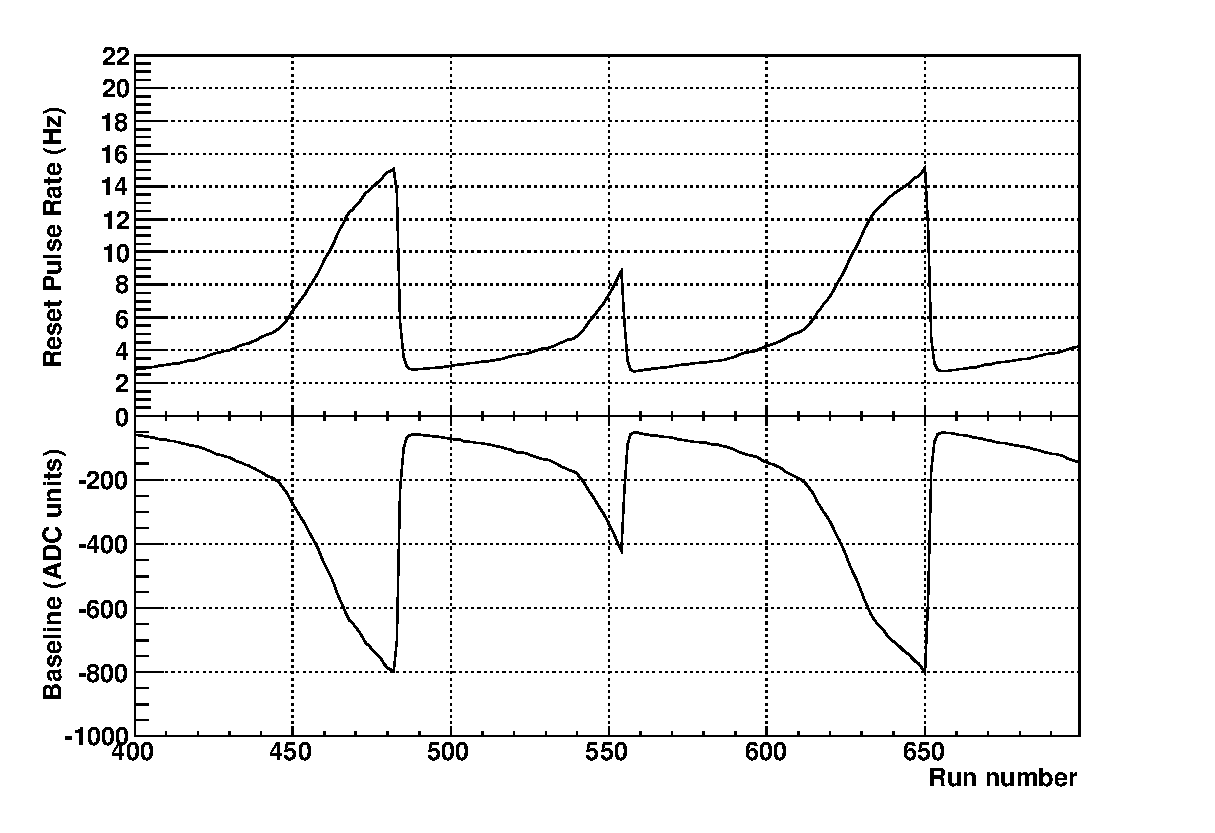
\includegraphics[width=0.9\textwidth]{BaselineVsRunNumberGraphPlot}
			%%%%	\caption{Measured baseline and inhibit rate versus run number for a subset of runs.}
			%%%%	\label{fig:PPC2BaselineInhibitRateVsTime}
			%%%%\end{figure}
						
				\begin{figure}
					\centering
					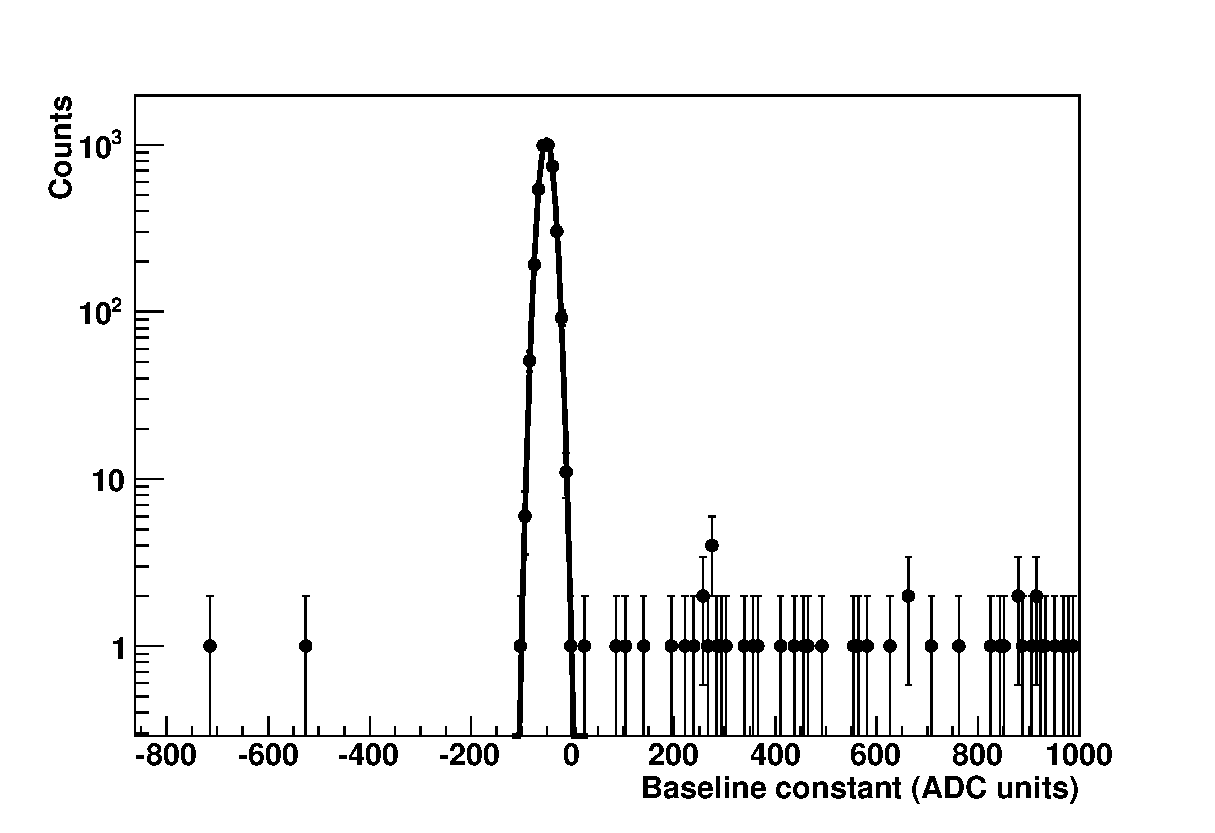
\includegraphics[width=0.7\textwidth]{BaselineExample}
					\caption[An example of a fit to the baseline for one hour-long run]
					{An example of a fit to the baseline for one hour-long run.  Line is a gaussian fit to the data.}
					\label{fig:PPC2BaselineCuts}
				\end{figure}
				
			\subsubsection{Integrated-counts-per-run cut}
	To determine the integrated-counts-per-run cut, counts in a designated energy window for each run were calculated and histogrammed.  The resulting data were then fit to a Poisson distribution and a cut was generated based upon 99.99\% acceptance using the fit distribution.  Results of this calculation are shown in Figure~\ref{fig:PPC2NoiseCuts}.  All runs with $\leq29$~counts between 0.6 and 10~keV were accepted.  
	
	All of these cuts were applied to the data to obtain a cleaned data set and all results described in the following sections use data after cuts.
	
				\begin{figure}
					\centering
					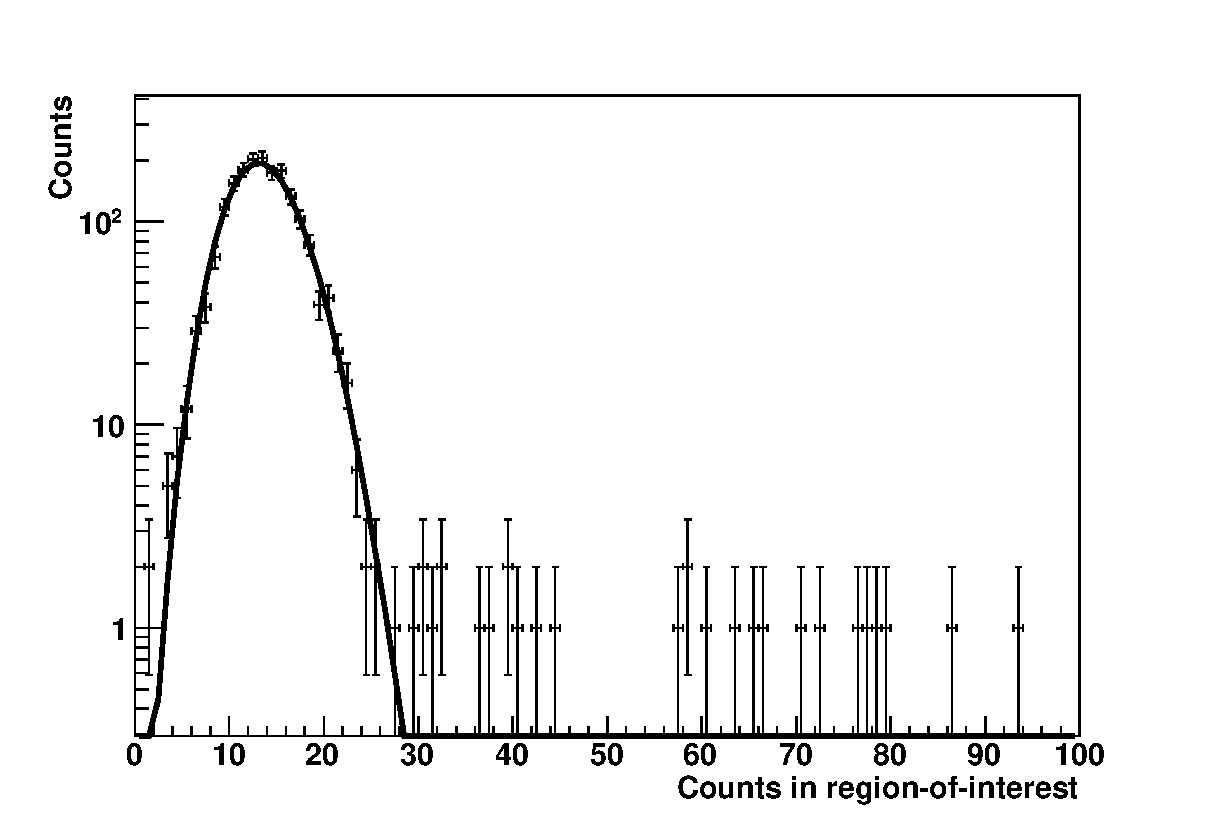
\includegraphics[width=0.7\textwidth]{LowROINoiseFit}
					\caption[Calculation of noise cuts]
					{Calculation of cut based upon the number of events in the energy window 0.6-10~keV per run.  
					The line is a fit to a Poisson distribution.  }
					\label{fig:PPC2NoiseCuts}
				\end{figure}
	
	    	\subsection{Rise-time calculations}
		\label{sec:DeploymentPPC2SoudanAnalysisRisetime}    
	
			
	The rise-time of each pulse was calculated using a simple algorithm: 
				\begin{enumerate}
					\item Subtract the baseline, $b$, and determine the amplitude, $a$.
					\item Forward search from beginning of the waveform to determine when the waveform reaches 
					$\frac{1}{2}a$ to find the middle of the pulse, $m$.
					\item From $m$, search backwards (forwards) to determine start (end) of the rise of the waveform.  
					The start and stop of the waveform are defined when the pulse reaches 10\% and 90\% of the amplitude.
				\end{enumerate}
The rise-time versus energy is plotted for each channel in Figure~\ref{fig:PPC2RisetimeCalculations}.  The low-gain channel demonstrates a sharp intensity at the $\sim$0.3~$\mu$s rise-time indicating that most pulses have this fast rise-time.  A number of gamma lines at higher energy are apparent in the data, including $^{40}$K (1460.8~keV), $^{214}$Bi (1764.5~keV), and $^{208}$Tl (2614.5~keV)\footnote{The thallium line is shifted in down in energy to $\sim$2550~keV.  An explanation of this is provided in Section~\ref{sec:DeploymentPPC2SoudanAnalysisEnergySpectra}}, with rise-time greater than~$0.3~\mu$s.  Because a large portion of events in these lines are composed of Compton-scatter interactions which deposit energy at multiple sites in the detector, this suggests multi-site events are being interpreted as slow-rise-time events.  
	
At low energy in the high-gain channel, one does not expect to see a significant multi-site population because Compton scatters summing to such a small energy are very improbable.  However, the rise-time distribution for the high-gain channel yields some interesting results: the strong line at $0.3~\mu$s still exists and there is a distribution near threshold ($\lesssim$1~keV) where it is clear the algorithm breaks down, but there is also a strong population of slow-rise-time events at low energy, $1\leq E \leq20$~keV.  Closer inspection reveals a significant visual difference between `fast' ($\sim$0.3~$\mu$s) pulses and `slow' ($>1~\mu$s) pulses as can been seen in Figure~\ref{fig:PPC2RisetimeExamplePulses}.  A similar result was found for this detector by J.~Orrell~\cite{Orrell}.  Since these slow-rise-time events are predominately at low energy, they can compose a background to any signal near threshold.  See Section~\ref{sec:RisetimeCuts} for discussion on improved identification and removal of these events including a discussion on their origin.
	
				\begin{figure}
					\centering
					\subfigure[High-gain channel.]{
						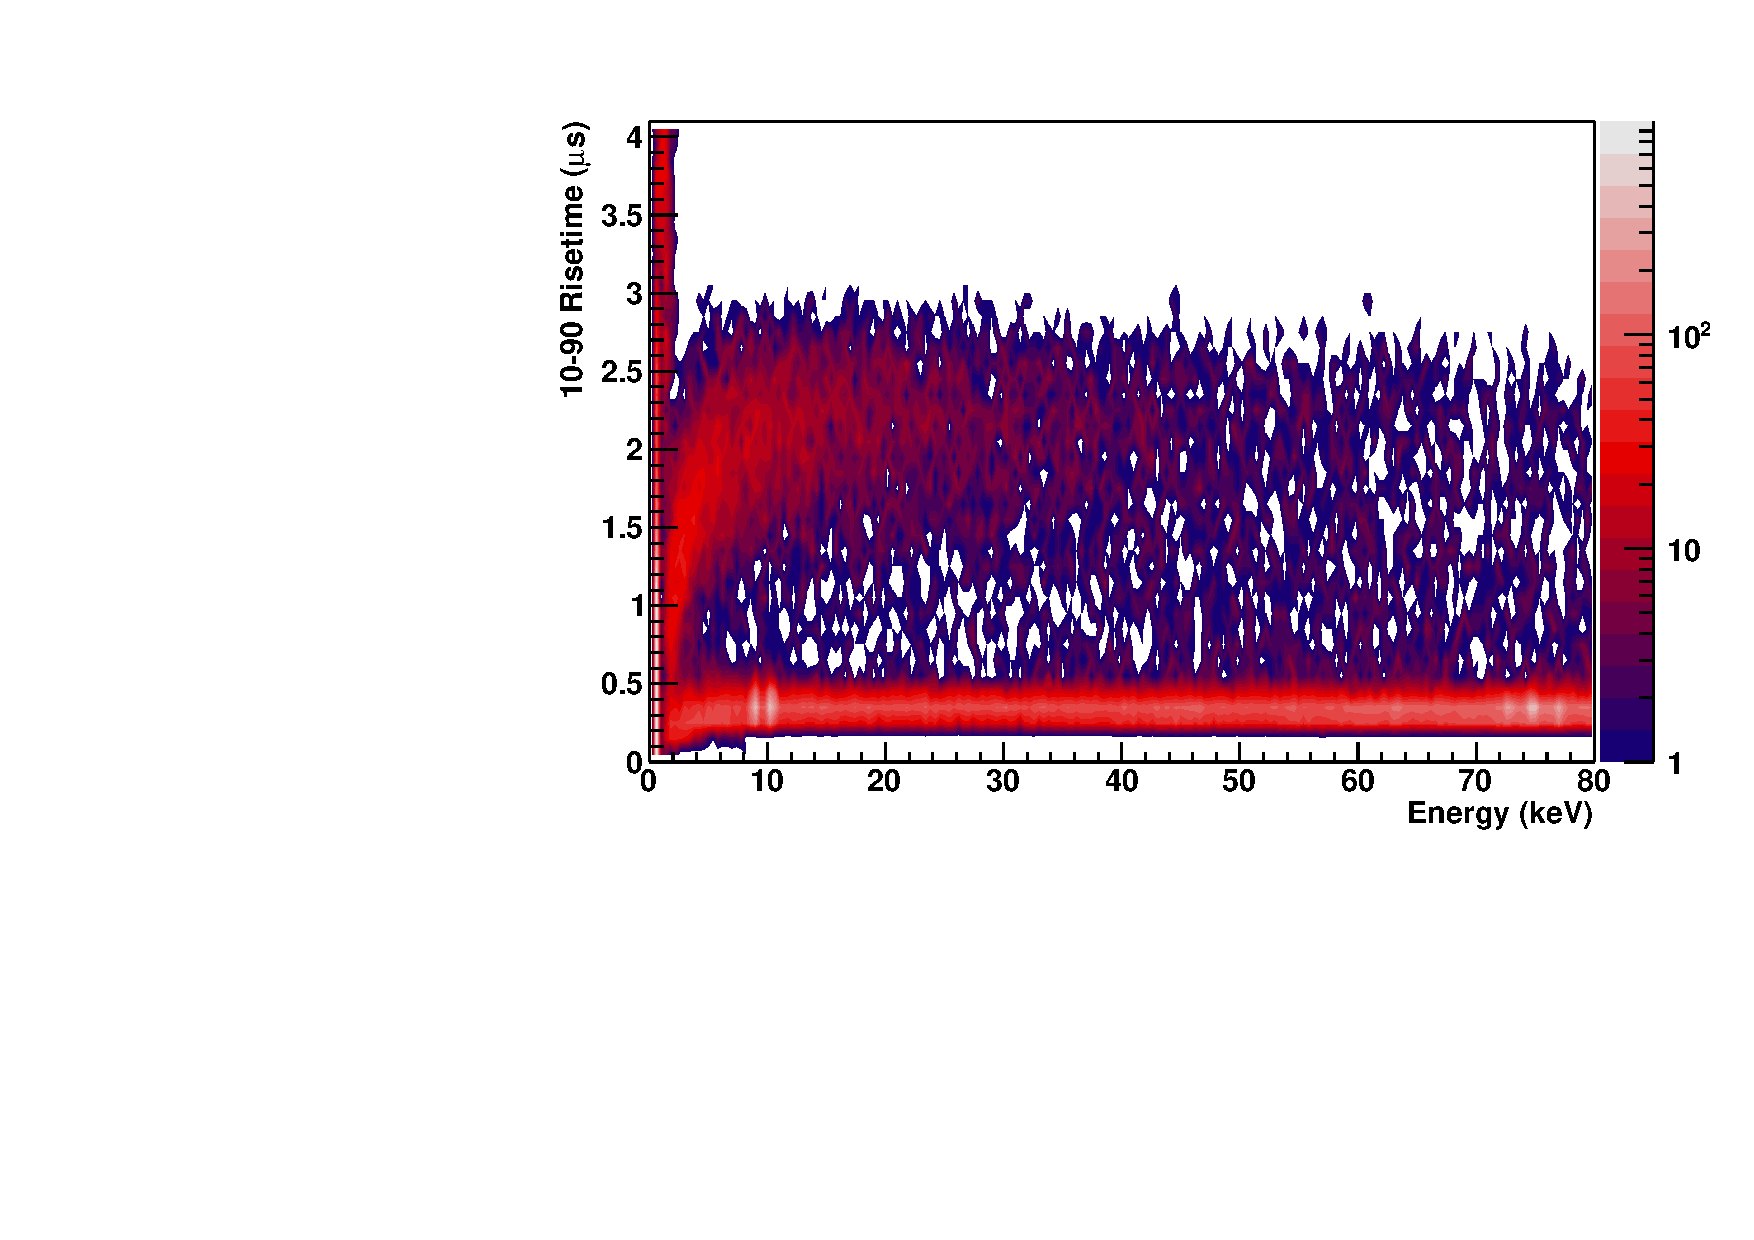
\includegraphics[width=0.8\textwidth]{RiseTimeVsEnergyChannel0}
						\label{fig:PPC2RisetimeCalculationsLow}
					}
					\subfigure[Low-gain channel.]{
						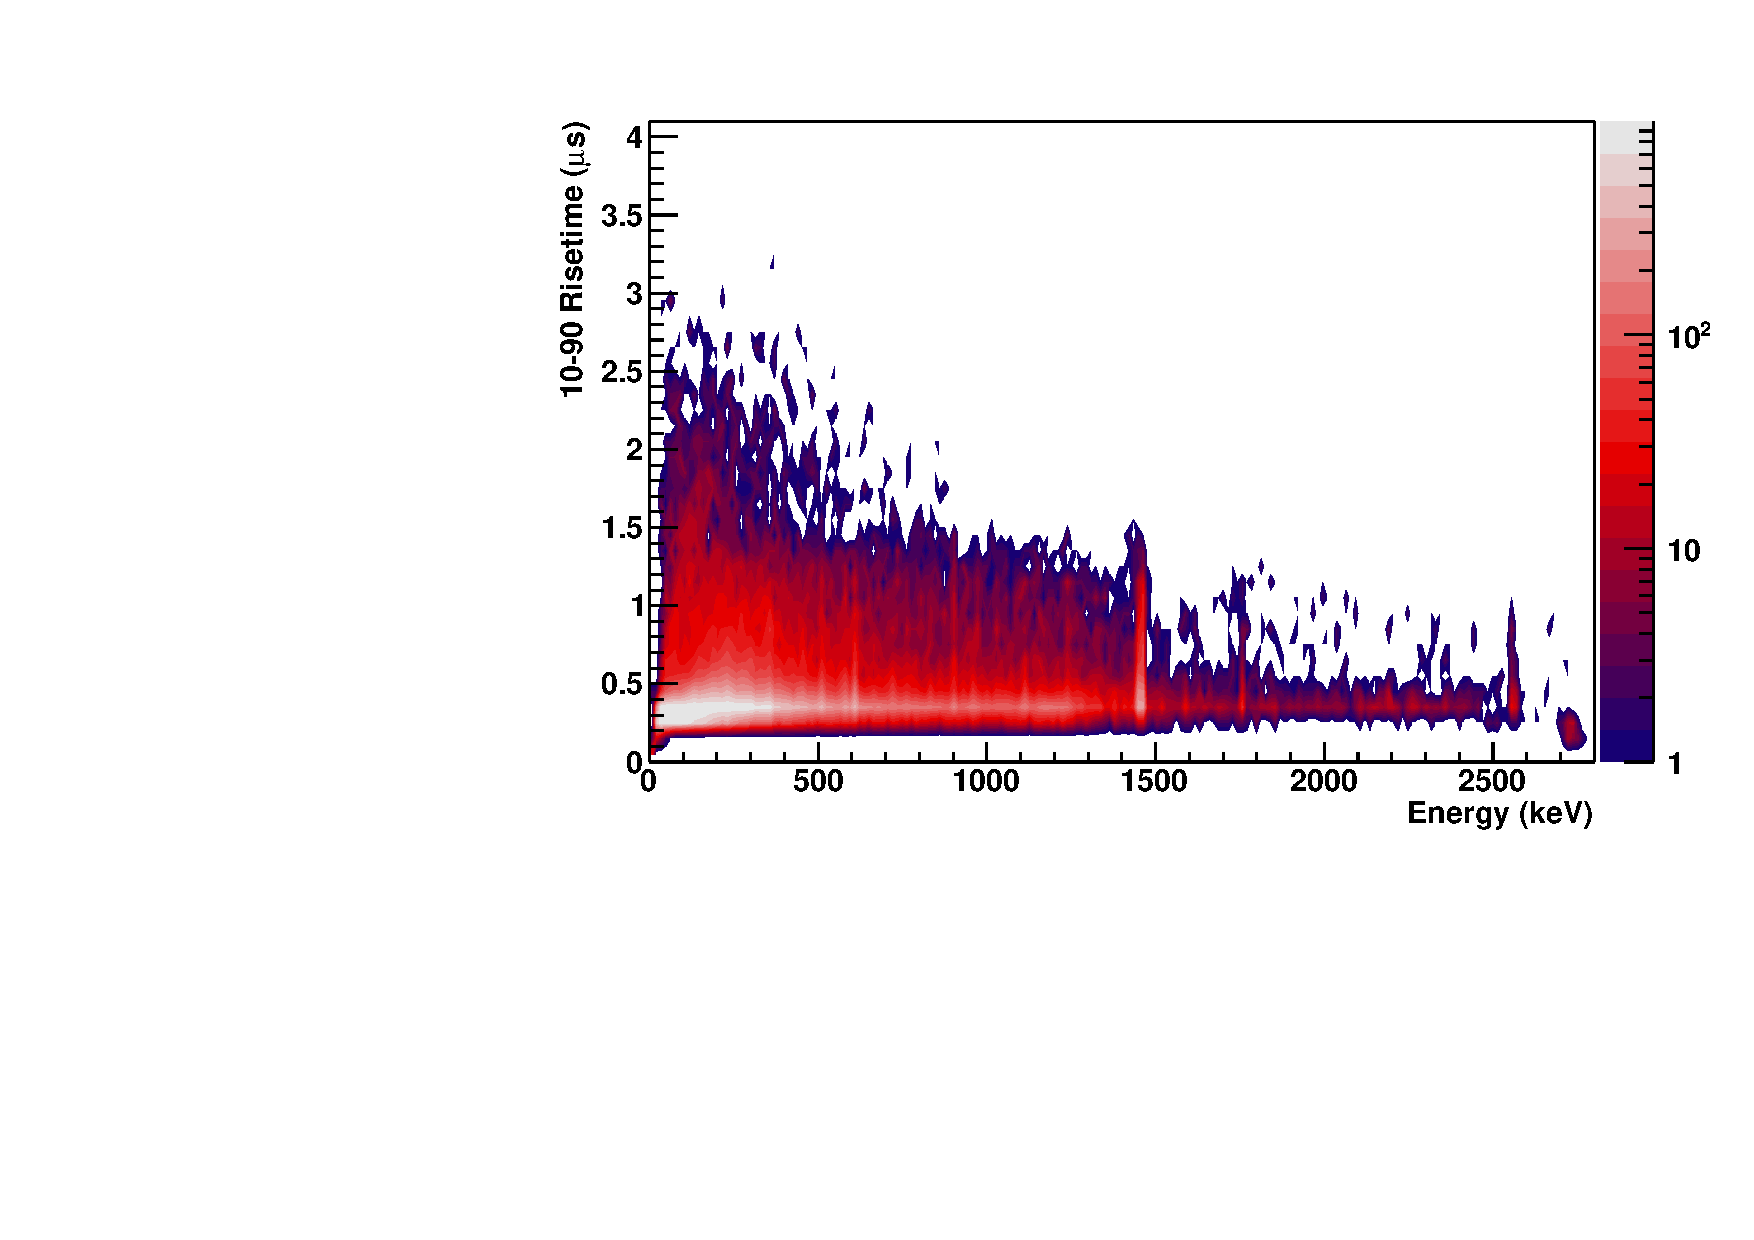
\includegraphics[width=0.8\textwidth]{RiseTimeVsEnergyChannel8}
						\label{fig:PPC2RisetimeCalculationsHigh}
					}	
					\caption[Rise-time measurements for high- and low-gain channels]
					{Risetime measurements for both high- and low-gain channels given in time from 10\%$\to$90\% 
					pulse amplitude.}
					\label{fig:PPC2RisetimeCalculations}
				\end{figure}		
	
				\begin{figure}
					\centering
					\subfigure[Fast pulse.]{
						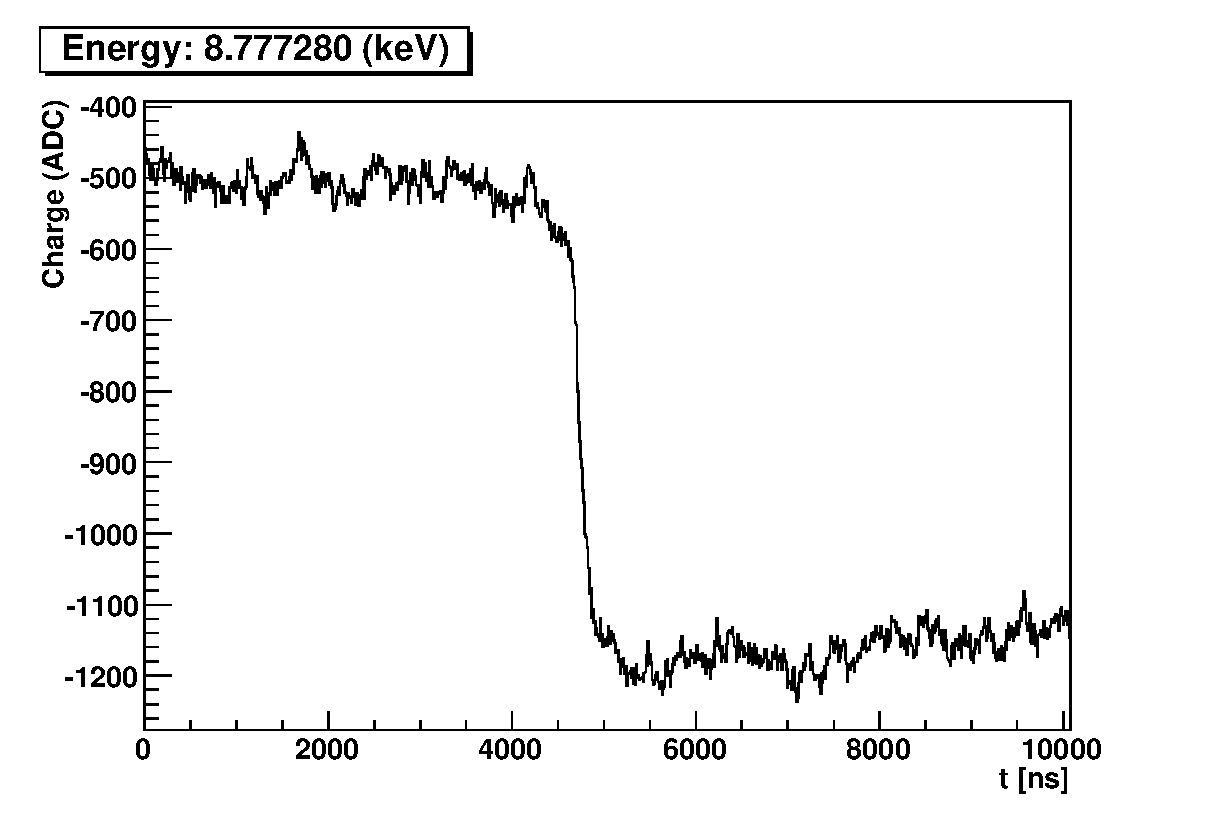
\includegraphics[width=0.45\textwidth]{fast_pulse_example}
						\label{fig:PPC2PulseExampleFast}
					}
					\subfigure[Slow pulse.]{
						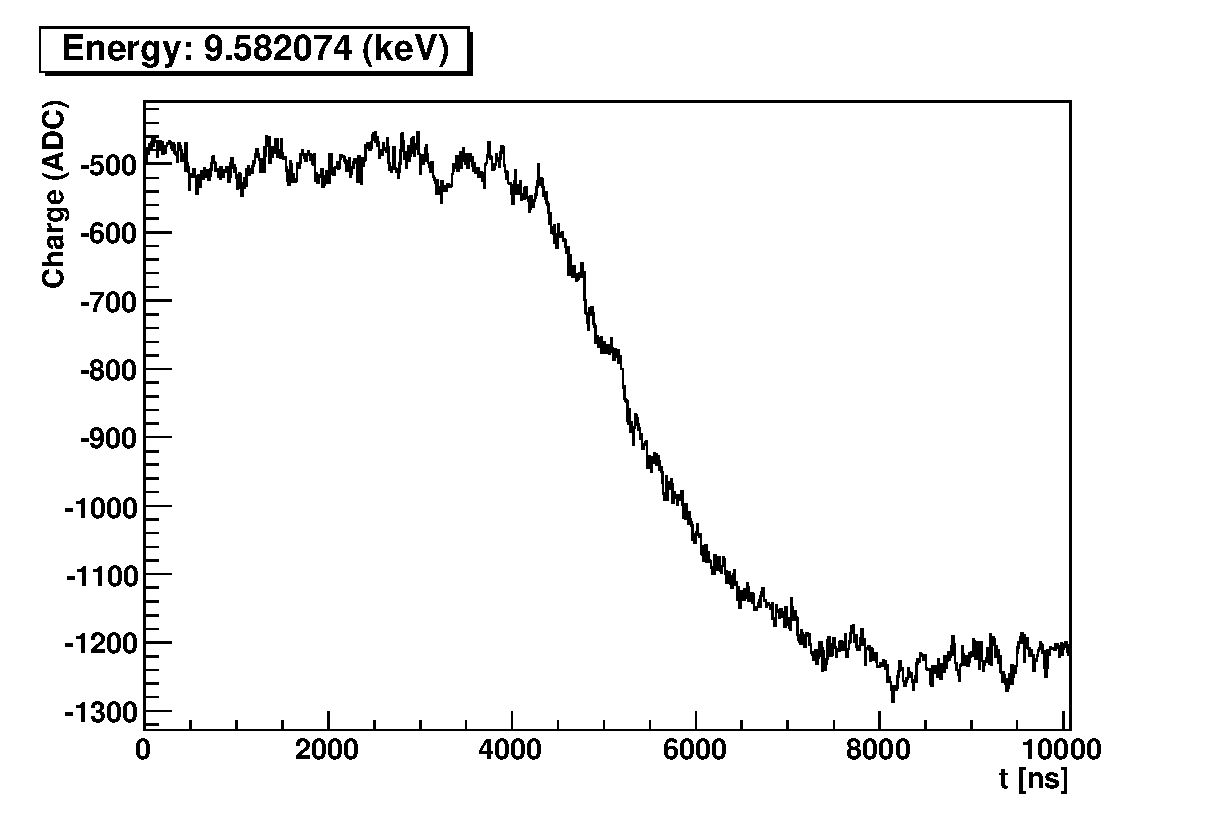
\includegraphics[width=0.45\textwidth]{slow_pulse_example}
						\label{fig:PPC2PulseExampleSlow}
					}					
					\caption[Examples of slow and fast rise-time pulses]
					{Examples of slow and fast rise-time pulses.}
					\label{fig:PPC2RisetimeExamplePulses}
				\end{figure}		
			
	    	\subsection{Energy spectra}
		\label{sec:DeploymentPPC2SoudanAnalysisEnergySpectra}    	
			
	Studies on the high-energy channel were performed by A.~Schubert to identify peaks and study the resolution of the detector with higher energy gamma lines~\cite{Schubert:2009ff}.  The spectrum was calibrated using prominent peaks in the spectra.  The resolution was fit to a second-order polynomial function of energy and determined to be:
				\begin{equation}
					\sigma = \sqrt{(0.242 \pm 0.016)^{2} +  E (4.04 \pm 0.1 \times 10^{-3})^{2} + E^{2} (9.2 \pm 0.0004 \times 10^{-4})^{2}} 
				\label{eqn:HighEnergySigma}
				\end{equation}			
with $E$, energy in keV.  It was found that the 2614.5~keV peak of the $^{208}$Tl decay was shifted down in energy to 2561~keV and had a larger-than-expected sigma (given Equation~\ref{eqn:HighEnergySigma}) of 8.6~keV.  This was explained by noting that large energy depositions in the crystal could saturate the pulse-reset preamp introducing either clipped or distorted pulses into the digitizer.  A selection of a few prominent lines fit in~\cite{Schubert:2009ff} is given in Table~\ref{tab:PPC2HighEnergyGammaLines}.  Results from this suggest that the linearity of the high-energy channel can not be trusted past the 1764~keV line of $^{214}$Bi.  This conclusion highlights a concern regarding the difficulty of using low-noise preamps with reset electronics while simultaneously looking at high-energy data $>$3-4~MeV as the \MJ~\minmod~will do.  Preamp solutions will have to address the optimization problem of ensuring enough dynamic range to search for $\nonubb$ while retaining low noise and threshold.  
	
				\begin{figure}
					\centering
					\subfigure[High-gain channel.]{
						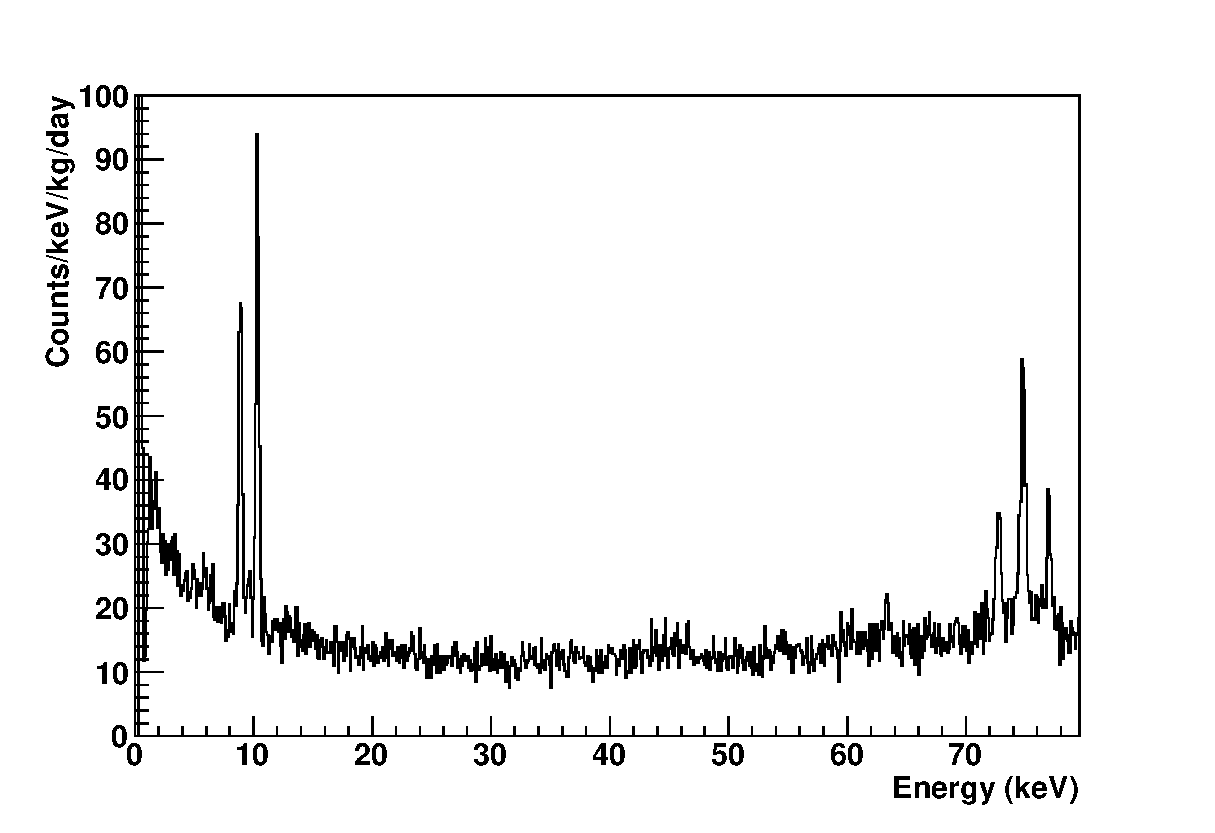
\includegraphics[width=0.8\textwidth]{LowEnergySpec}
						\label{fig:PPC2EnergySpecLow}
					}
					\subfigure[Low-gain channel.]{
						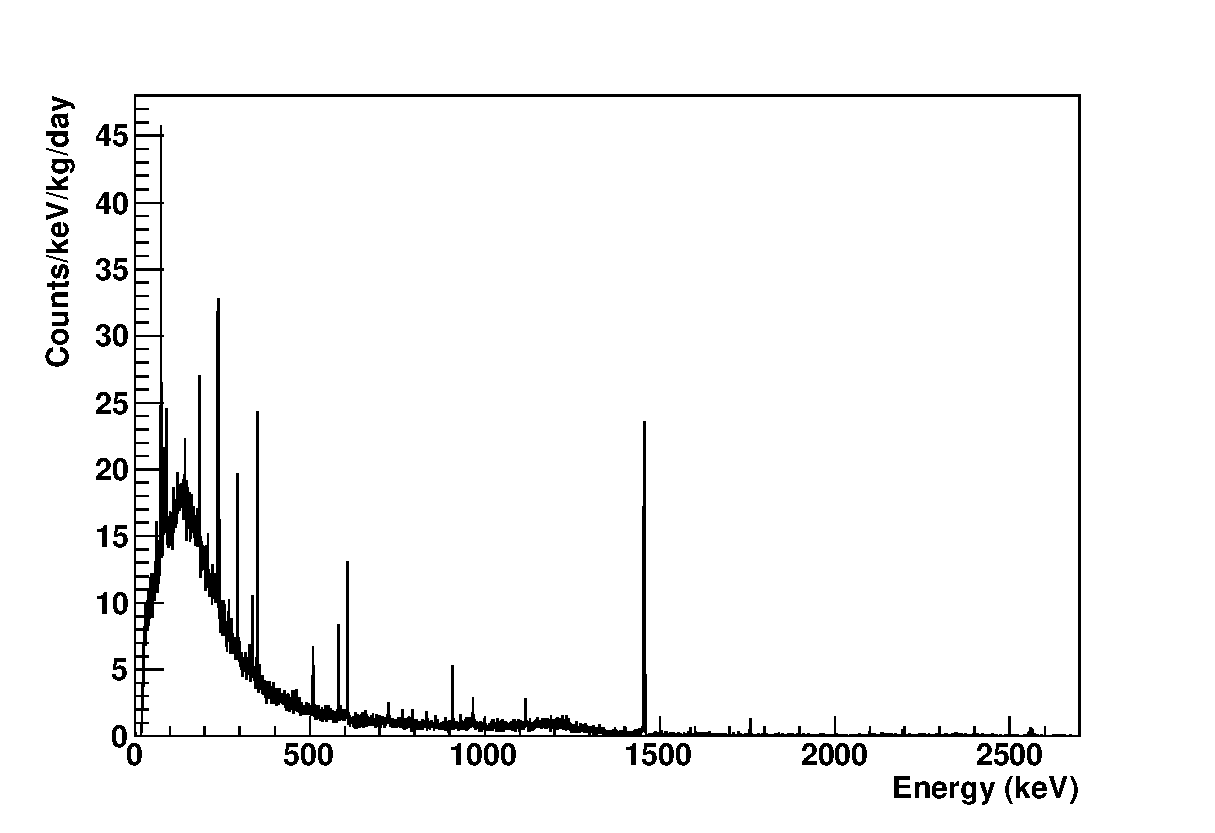
\includegraphics[width=0.8\textwidth]{HighEnergySpec}
						\label{fig:PPC2EnergySpecHigh}
					}
					\caption[Energy spectra of PPC2]
					{Energy spectra of PPC2.}
					\label{fig:PPC2EnergySpectra}
				\end{figure}	
	
				\begin{table}
					\centering
					\begin{tabular}{  c | r | r | c  }
					\hline
					{\bf Source} & {\bf Energy [keV]} & {\bf Fit centroid [keV]} & {\bf Sigma [keV]} \\  
					\hline
					% fit of 1-degree polynomial continuum + 0 sawtooths + 1 gaussian(s) without  tail(s), wit\\
					$^{226}$Ra     & 186.2     ~ & 185.7      ${\pm}$ 0.04       ~ & 0.37       ${\pm}$ 0.03       \\
					% fit of 1-degree polynomial continuum + 0 sawtooths + 3 gaussian(s) without  tail(s), wit\\
					$^{212}$Pb     & 238.6     ~ & 238.5      ${\pm}$ 0.04       ~ & 0.32       ${\pm}$ 0.01       \\
					% fit of 1-degree polynomial continuum + 0 sawtooths + 3 gaussian(s) without  tail(s), wit\\
					$^{214}$Pb     & 242.0     ~ & 241.9      ${\pm}$ 0.04       ~ & 0.30       ${\pm}$ 0.06       \\
					% fit of 1-degree polynomial continuum + 0 sawtooths + 1 gaussian(s) without  tail(s), wit\\
					$^{214}$Pb     & 295.2     ~ & 295.1      ${\pm}$ 0.04       ~ & 0.41       ${\pm}$ 0.02       \\
					% fit of 1-degree polynomial continuum + 0 sawtooths + 1 gaussian(s) without  tail(s), wit\\
					$^{228}$Ac     & 338.3     ~ & 338.1      ${\pm}$ 0.04       ~ & 0.42       ${\pm}$ 0.04       \\
					% fit of 1-degree polynomial continuum + 0 sawtooths + 1 gaussian(s) without  tail(s), wit\\
					$^{214}$Pb     & 351.9     ~ & 351.7      ${\pm}$ 0.04       ~ & 0.38       ${\pm}$ 0.01       \\
					% fit of 1-degree polynomial continuum + 0 sawtooths + 1 gaussian(s) without  tail(s), wit\\
					$^{208}$Tl     & 583.2     ~ & 583.5      ${\pm}$ 0.04       ~ & 0.58       ${\pm}$ 0.03       \\
					% fit of 1-degree polynomial continuum + 0 sawtooths + 1 gaussian(s) without  tail(s), wit\\
					$^{214}$Bi     & 609.3     ~ & 609.6      ${\pm}$ 0.04       ~ & 0.60       ${\pm}$ 0.02       \\
					% fit of 1-degree polynomial continuum + 0 sawtooths + 1 gaussian(s) without  tail(s), wit\\
					$^{228}$Ac     & 911.2     ~ & 911.6      ${\pm}$ 0.1       ~ & 0.71       ${\pm}$ 0.06       \\
					% fit of 1-degree polynomial continuum + 0 sawtooths + 1 gaussian(s) without  tail(s), wit\\
					% fit of 1-degree polynomial continuum + 0 sawtooths + 1 gaussian(s) without  tail(s), wit\\
					$^{228}$Ac     & 969.0     ~ & 969.3      ${\pm}$ 0.1       ~ & 0.79       ${\pm}$ 0.10       \\
					% fit of 1-degree polynomial continuum + 0 sawtooths + 1 gaussian(s) without  tail(s), wit\\
					$^{214}$Bi     & 1120.3    ~ & 1120.5     ${\pm}$ 0.1       ~ & 1.03       ${\pm}$ 0.11       \\
					% fit of 1-degree polynomial continuum + 0 sawtooths + 1 gaussian(s) without  tail(s), wit\\
					$^{40}$K       & 1460.8    ~ & 1460.7     ${\pm}$ 0.04       ~ & 1.33       ${\pm}$ 0.02       \\
					% fit of 1-degree polynomial continuum + 0 sawtooths + 1 gaussian(s) without  tail(s), wit\\
					$^{214}$Bi     & 1764.5    ~ & 1764.3     ${\pm}$ 0.2       ~ & 1.72       ${\pm}$ 0.22       \\
					% sigma = sqrt( A^2 + energy*B^2 + energy^2*B^2 )\\
					% A = 1.8463 +/- 0.1859 E-1\\
					% B = 1.0921 +/- 0.2098 E-2\\
					% C = 8.4401 +/- 0.2725 E-4\\
					% 26 peaks were fit\\
					% chi-squared/dof: 83.3478 / 23.0000 ( 3.6238), p-val: 9.0378E-9\\
					% fit of 1-degree polynomial continuum + 0 sawtooths + 1 gaussian(s) without  tail(s), wit\\
					$^{214}$Bi     & 2204.2    ~ & 2201.5     ${\pm}$ 0.5       ~ & 1.94       ${\pm}$ 0.36       \\
					% sigma = sqrt( A^2 + energy*B^2 + energy^2*B^2 )\\
					% A = 1.8464 +/- 0.1857 E-1\\
					% B = 1.0918 +/- 0.2094 E-2\\
					% C = 8.4406 +/- 0.2711 E-4\\
					% 27 peaks were fit\\
					% chi-squared/dof: 83.3481 / 24.0000 ( 3.4728), p-val: 1.7660E-8\\
					% fit of 1-degree polynomial continuum + 0 sawtooths + 1 gaussian(s) without  tail(s), wit\\
					$^{208}$Tl    & 2614.5    ~ & 2560.6     ${\pm}$ 0.8       ~ & 8.59       ${\pm}$ 0.70       \\
					% fit of 1-degree polynomial continuum + 0 sawtooths + 1 gaussian(s) without  tail(s), wit\\
					% sigma = sqrt( A^2 + energy*B^2 + energy^2*B^2 )\\
					% A = 1.9182 +/- 0.1804 E-1\\
					% B = 9.5840 +/- 2.3753 E-3\\
					% C = 8.6656 +/- 0.2641 E-4\\
					% 29 peaks were fit\\
					% chi-squared/dof: 217.5429 / 26.0000 ( 8.3670), p-val: 3.7087E-32\\
					\hline
					\end{tabular}

				
					\caption[Selection of gamma lines in the high-energy channel of PPC2]
					{Selection of gamma lines in the high-energy channel of PPC2.  Table courtesy A.~Schubert.}
					\label{tab:PPC2HighEnergyGammaLines}
				\end{table}
	
	The calibration of the low-energy channel was refined using the \gersixeight~and \znsixfive~K-capture lines plus the non-overlapping x-ray lines from Pb and Bi.  The final maximum likelihood fits to these lines, means and sigmas and their expected value, are given in Table~\ref{tab:PPCLowEnergyLines}.  The x-ray lines from Pb and Bi come from the $\beta$-decays of $^{208}$Tl and $^{214}$Pb in the $^{232}$Th and $^{238}$U decay chains.  The two lines at $\sim$73~keV were fit with one gaussian which generated a wider width.  
				\begin{table}
					\begin{tabular}{l|c|c|c}
						Source & Energy (keV) & Fit Mean (keV) & Fit Sigma (eV) \\
						\hline						
						\znsixfive~K-capture & 8.979 & 8.95$\pm7.6\times10^{-3}$ & $139 \pm 7.3$ \\
						\hline
						\gersixeight~K-capture & 10.367 & $10.394\pm5.8\times10^{-3}$ & $119 \pm 7.3$ \\
						\hline
						$^{(208)}$Pb K$_{\alpha2}$ & 72.805 & $72.86\pm2.1\times10^{-2}$ & $188 \pm 19.7$ \\
						\hline
						$^{(208)}$Pb K$_{\alpha1}$, $^{(214)}$Ba K$_{\alpha2}$ & 74.969, 74.815 & $74.92\pm1.3\times10^{-2}$ & $234 \pm 19.7$ \\
						\hline
						$^{(214)}$Ba K$_{\alpha1}$ & 77.107& $77.11\pm1.9\times10^{-2}$ & $163 \pm 19.7$ \\				
						\hline																
					\end{tabular}
					\caption[Lines in the low-energy channel of PPC2]
					{Lines in the low-energy channel of PPC2.}
					\label{tab:PPCLowEnergyLines}
				\end{table}

	\section{Estimate of \gersixeight~surface production}       
	\label{sec:Ge68ProdPPC}
	
       \gersixeight~is a cosmogenically-produced isotope inside germanium detectors which is a well-known background to $\nonubb$ (see e.g.~\cite{Ceb06aa}) due to the fact that the decays of its \galsixeight~daughters can deposit energy in the $\nonubb$ region-of-interest.  A schematic of the decay chain is shown in Figure~\ref{fig:GE68Decay}.  The initial decay of \gersixeight~proceeds via electron-capture with a half-life of 271~days to \galsixeight, which subsequently decays to $^{68}$Zn with a half-life of 68~minutes.  The latter decay has a Q-value of 2921~keV which could deposit energy at 2039~keV, the $\nonubb$ Q-value.  This background can be reduced two ways: (1) an analysis cut which tags the initial decay of \gersixeight~and vetoes the detector for a specified multiple of \galsixeight~half-lives, and/or (2) reduce the intrinsic \gersixeight~content in germanium detectors by either storing them in a low-cosmic-ray-flux environment (i.e.~underground) and waiting or by actively removing \gersixeight~through isotopic depletion.  Because \gersixeight~decays inside the detector, the total energy emitted through Auger electrons and x-rays is summed to lines of the K-, L-, or M-electron binding energy of the daughter nuclei (see Table~\ref{tab:GE68decayinfo}).  These lines can then be used to tag events likely to belong to a \gersixeight~decay.  Tagging the \gersixeight~decays to reduce the \galsixeight~background is dependent on the decay rate of \gersixeight, $\lambda^{(^{68}Ge)}$, and is not a viable solution until $\lambda^{(^{68}Ge)} \tau_{1/2}^{(^{68}Ga)} \ll 1$.   Estimations of the \gersixeight~activation rate at the earth's surface in both natural and enriched (86\% $^{76}$Ge) have been performed previously (see e.g.~\cite{Avi92,Elliott:2009cw}).  

       
       			\begin{table}
				\centering
				\begin{tabular}{|l|c|r|}
					\hline
					\gersixeight~decays & Percent & Energy (keV) \\
					\hline
					     K-capture & $86.25\pm0.22$\% & 10.367 \\
					     L-capture & $11.45\pm0.20$ \% & 1.299 \\
					     M-capture & $1.92\pm0.08$\% & $\sim$0.1 \\
					\hline
				\end{tabular}
				\caption[Decay information of\ \gersixeight]
				{Decay information of\ \gersixeight.  Capture probabilities are adapted from 
				reference~\cite{Schonfeld1994955}, characteristic energies from~\cite{Bea67}.}
				\label{tab:GE68decayinfo}
			\end{table}	
			\begin{figure}
				\centering
				\begin{tikzpicture}[node distance=0.4\textwidth]
		    			\node[circle] (GE68) {$^{68}$Ge};
					\node[circle, right of=GE68] (ga68) {$^{68}$Ga};
					\node[circle, right of=ga68] (zn68) {$^{68}$Zn};
					    
					\path[draw,->] (GE68) -- node[above] {\scriptsize $\epsilon$, T$_{1/2}=$271~d} (ga68);
					\path[draw,->] (ga68) -- node[above] {\scriptsize $\epsilon$, T$_{1/2}=$68~m, Q=2921~keV} (zn68);
					\draw (ga68) node[draw, rectangle, color=red, minimum height=0.1\textheight, minimum width=0.9\textwidth] {};
		 		\end{tikzpicture}
				\caption[Decay chain of $^{68}$Ge]
				{Decay chain of $^{68}$Ge.}
				\label{fig:GE68Decay}
			\end{figure}
			      
     The PPC2 detector provided an excellent opportunity to measure the \gersixeight~activation rate at the surface.  Though the background rate at the L-capture energy of \gersixeight~was too high to resolve any peak, the K-capture line at 10.367~keV provided a means to measure the activation rate.  At the surface, the detector was assumed to be at equilibrium: that is, the decay rate of the cosmogenic isotopes were equal to the population rates.  This was a good approximation since the detector had been kept at the surface for a period on the order of the lifetime of \gersixeight.  Once the detector is brought underground, the cosmogenic isotopes are being populated at a rate much lower than that at the surface and it is a safe to assume at the depths of Soudan ($\sim2000$~m.w.e.) that this rate is 0.  Therefore, an underground measurement of the decay rate of \gersixeight~in counts/day can be used to determine the activation rate in counts/day at the surface.  The measurement was performed after \gersevenone, a short-lived cosmogenic ($\tau_{1/2}=11.4$~days) which also populates the same capture peaks, had decayed.  
		
	To perform the measurement, an energy window was selected around the K-capture peak from 10$\to$10.73~keV as the ``signal'' region -- chosen as symmetric around the expected signal mean -- and from 11$\to$15 as the ``background'' region, nearby and without any x-ray lines.  The average rate, in counts/keV/kg/day, was computed for each 72~hours of live-time in both regions and fit simultaneously to the function:
	
			\begin{equation}
				f(E,t) = \left\{ 
				\begin{array}{lr} 
 					a + b e^{-\left( \log{2} \right) t/\tau_{1/2}} & 10 \leq E \leq 10.73~\textrm{(keV)}\\
					\\
					a & 11 \leq E \leq 15~\textrm{(keV)}\\
				\end{array} \right.			
			\end{equation}
with the free parameters $a$ (flat background rate), $b$ (\gersixeight~rate), and $\tau_{1/2}$ (\gersixeight~half-life).  Fit results of this are summarized in Table~\ref{tab:Ge68FitResults} and plotted in Figure~\ref{fig:GE68Production}.  At the beginning of the counting runs, the detector had already been underground 212~days, meaning that the estimated decay rate, $b$, must be multiplied by the value $e^{(\log(2)~212 d/270.95 d)} = 1.72$ as well as  the energy window (0.73~keV) to get the counts-per-day-per-kilogram the day the detector was brought underground.  It was necessary to estimate the acceptance of the energy window using parameters ($\mu$ and $\sigma$) found from a maximum likelihood fit to the data (see, e.g.~Section~\ref{sec:DeploymentPPC2SoudanAnalysisEnergySpectra}); this acceptance was measured as $0.99797\pm0.001$.  Finally, since only the K-capture line was used in this estimation, the percentage of decays into this channel must be taken into account (see Table~\ref{tab:GE68decayinfo}).  The final result was then determined to be $53.3\pm4.3$~counts/kg/day which can also be interpreted as the activation rate for \gersixeight.  A comparison of this value to previous results is given in Table~\ref{tab:Ge68PreviousResults}.

       			\begin{table}
				\centering
				\begin{tabular}{l|r}
					\hline
					Parameter & Fit Value \\
					\hline
					$a$ & $16.166\pm0.33$ (counts/keV/kg/d)  \\
					$b$ & $36.54\pm2.94$ (counts/keV/kg/d)  \\
					$\tau_{1/2}$ & $192\pm96$ (days) \\
					$\chi^{2}$/NDF & 32.3/45 \\					
					\hline
				\end{tabular}
				\caption[Fit information for \gersixeight~analysis]
				{Fit information for \gersixeight~analysis.}
				\label{tab:Ge68FitResults}	
			\end{table}	
			
			\begin{figure}
				\centering
				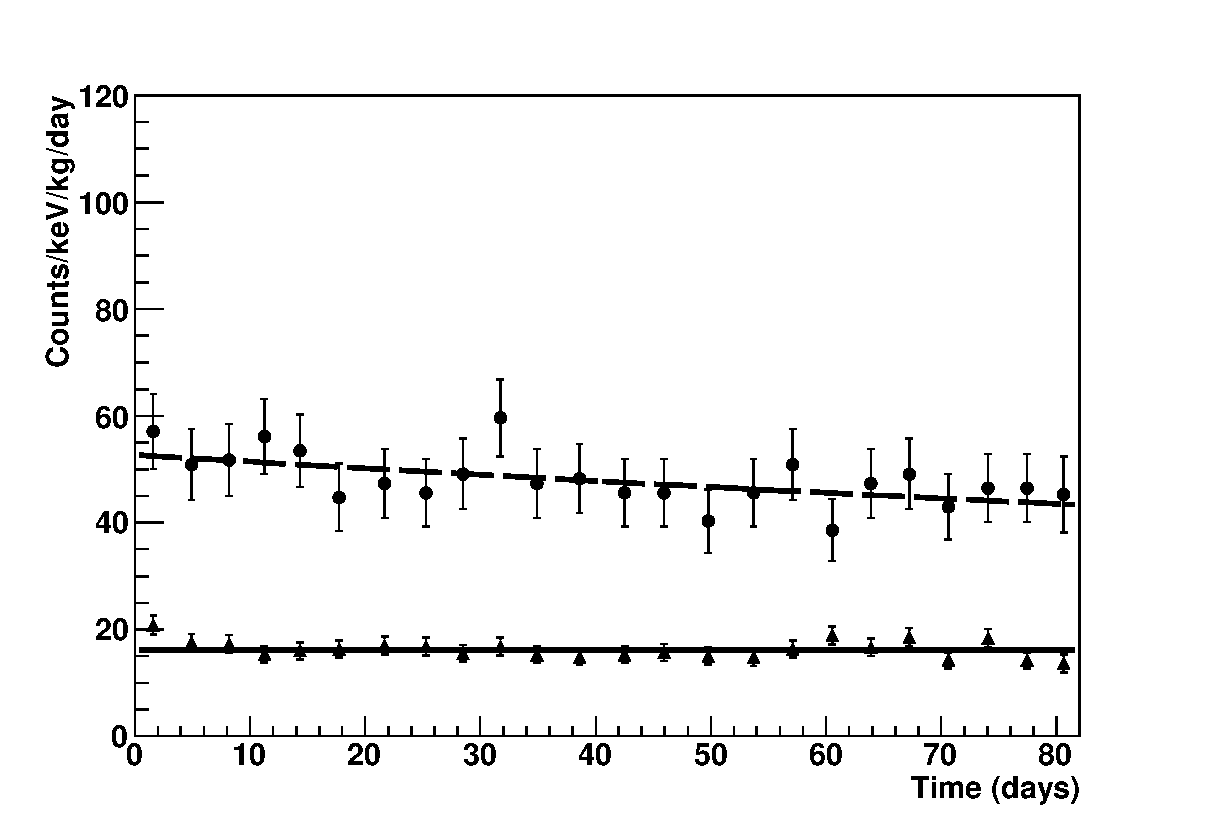
\includegraphics[width=0.7\textwidth]{G68_results}
				\caption[Estimation of $^{68}$Ge production at the surface]
				{Estimation of $^{68}$Ge production at the surface.  Data and fit for two regions:
				(1) 10$\to$10.73~keV, fit to exponential + constant (circles); and (2) 11$\to$14~keV, 
				fit to constant (triangles).  See text for fit details.}
				\label{fig:GE68Production}
			\end{figure}			
			
	          
	          	\begin{table}
				\caption[Summary of previous estimates of \gersixeight~surface activation rates]
				{A summary of previous estimates of \gersixeight~surface activation rates, 
				adapted from~\cite{Elliott:2009cw}.}
				\label{tab:Ge68PreviousResults}
	          	\end{table}			
			
	\section{Conclusions}
	
	A \MJ-like data acquisition system operated stably in a deployed environment for over a half year, demonstrating software and hardware robustness required for the \MJ~\minmod.  A tiered analysis framework was constructed, allowed automated processing and management of data from the deployed system.  This flexible framework was applied to data from two other detectors, including one analyzed in Chapter~\ref{chap:AnalysisBeGe}.  Several parameters of the data were tracked and exhibited deviations over time, underscoring the need to monitor channel rates, electronic noise, and trigger efficiency throughout the life of a deployed system.  Though the backgrounds seen in the detector were too large to provide competitive limits on dark matter signals, two important results from the data were made including a measurement of rise-time versus energy for low-energy pulses and an estimation of \gersixeight~surface activation in natural germanium.  The measurement of the former determined a potential source of background for applications such as the \MJ~\minmod~using PPCs for direct dark matter detection.  Results from this deployment reaffirmed conclusions made in Chapter~\ref{chap:DAQDevel}, namely that the trigger efficiency and electronic noise measured with this system were insufficient and would require an update in hardware for improvement.

